\chapter{UYGULAMA VE BULGULAR}

Aura Finance uygulaması, geliştirilen mimari ve algoritmaların birleşimiyle tam fonksiyonel bir finansal yönetim platformu olarak hayata geçirilmiştir. Bu bölümde, uygulamanın kullanıcı arayüzü ve elde edilen bulgular ekran görüntüleri eşliğinde sunulmaktadır.

\section{Kullanıcı Arayüzü Analizi}

Uygulamanın arayüzü, kullanıcı deneyimini (UX) ön planda tutan modern ve responsive bir yapıdadır.

\begin{figure}[h!]
 \centering
 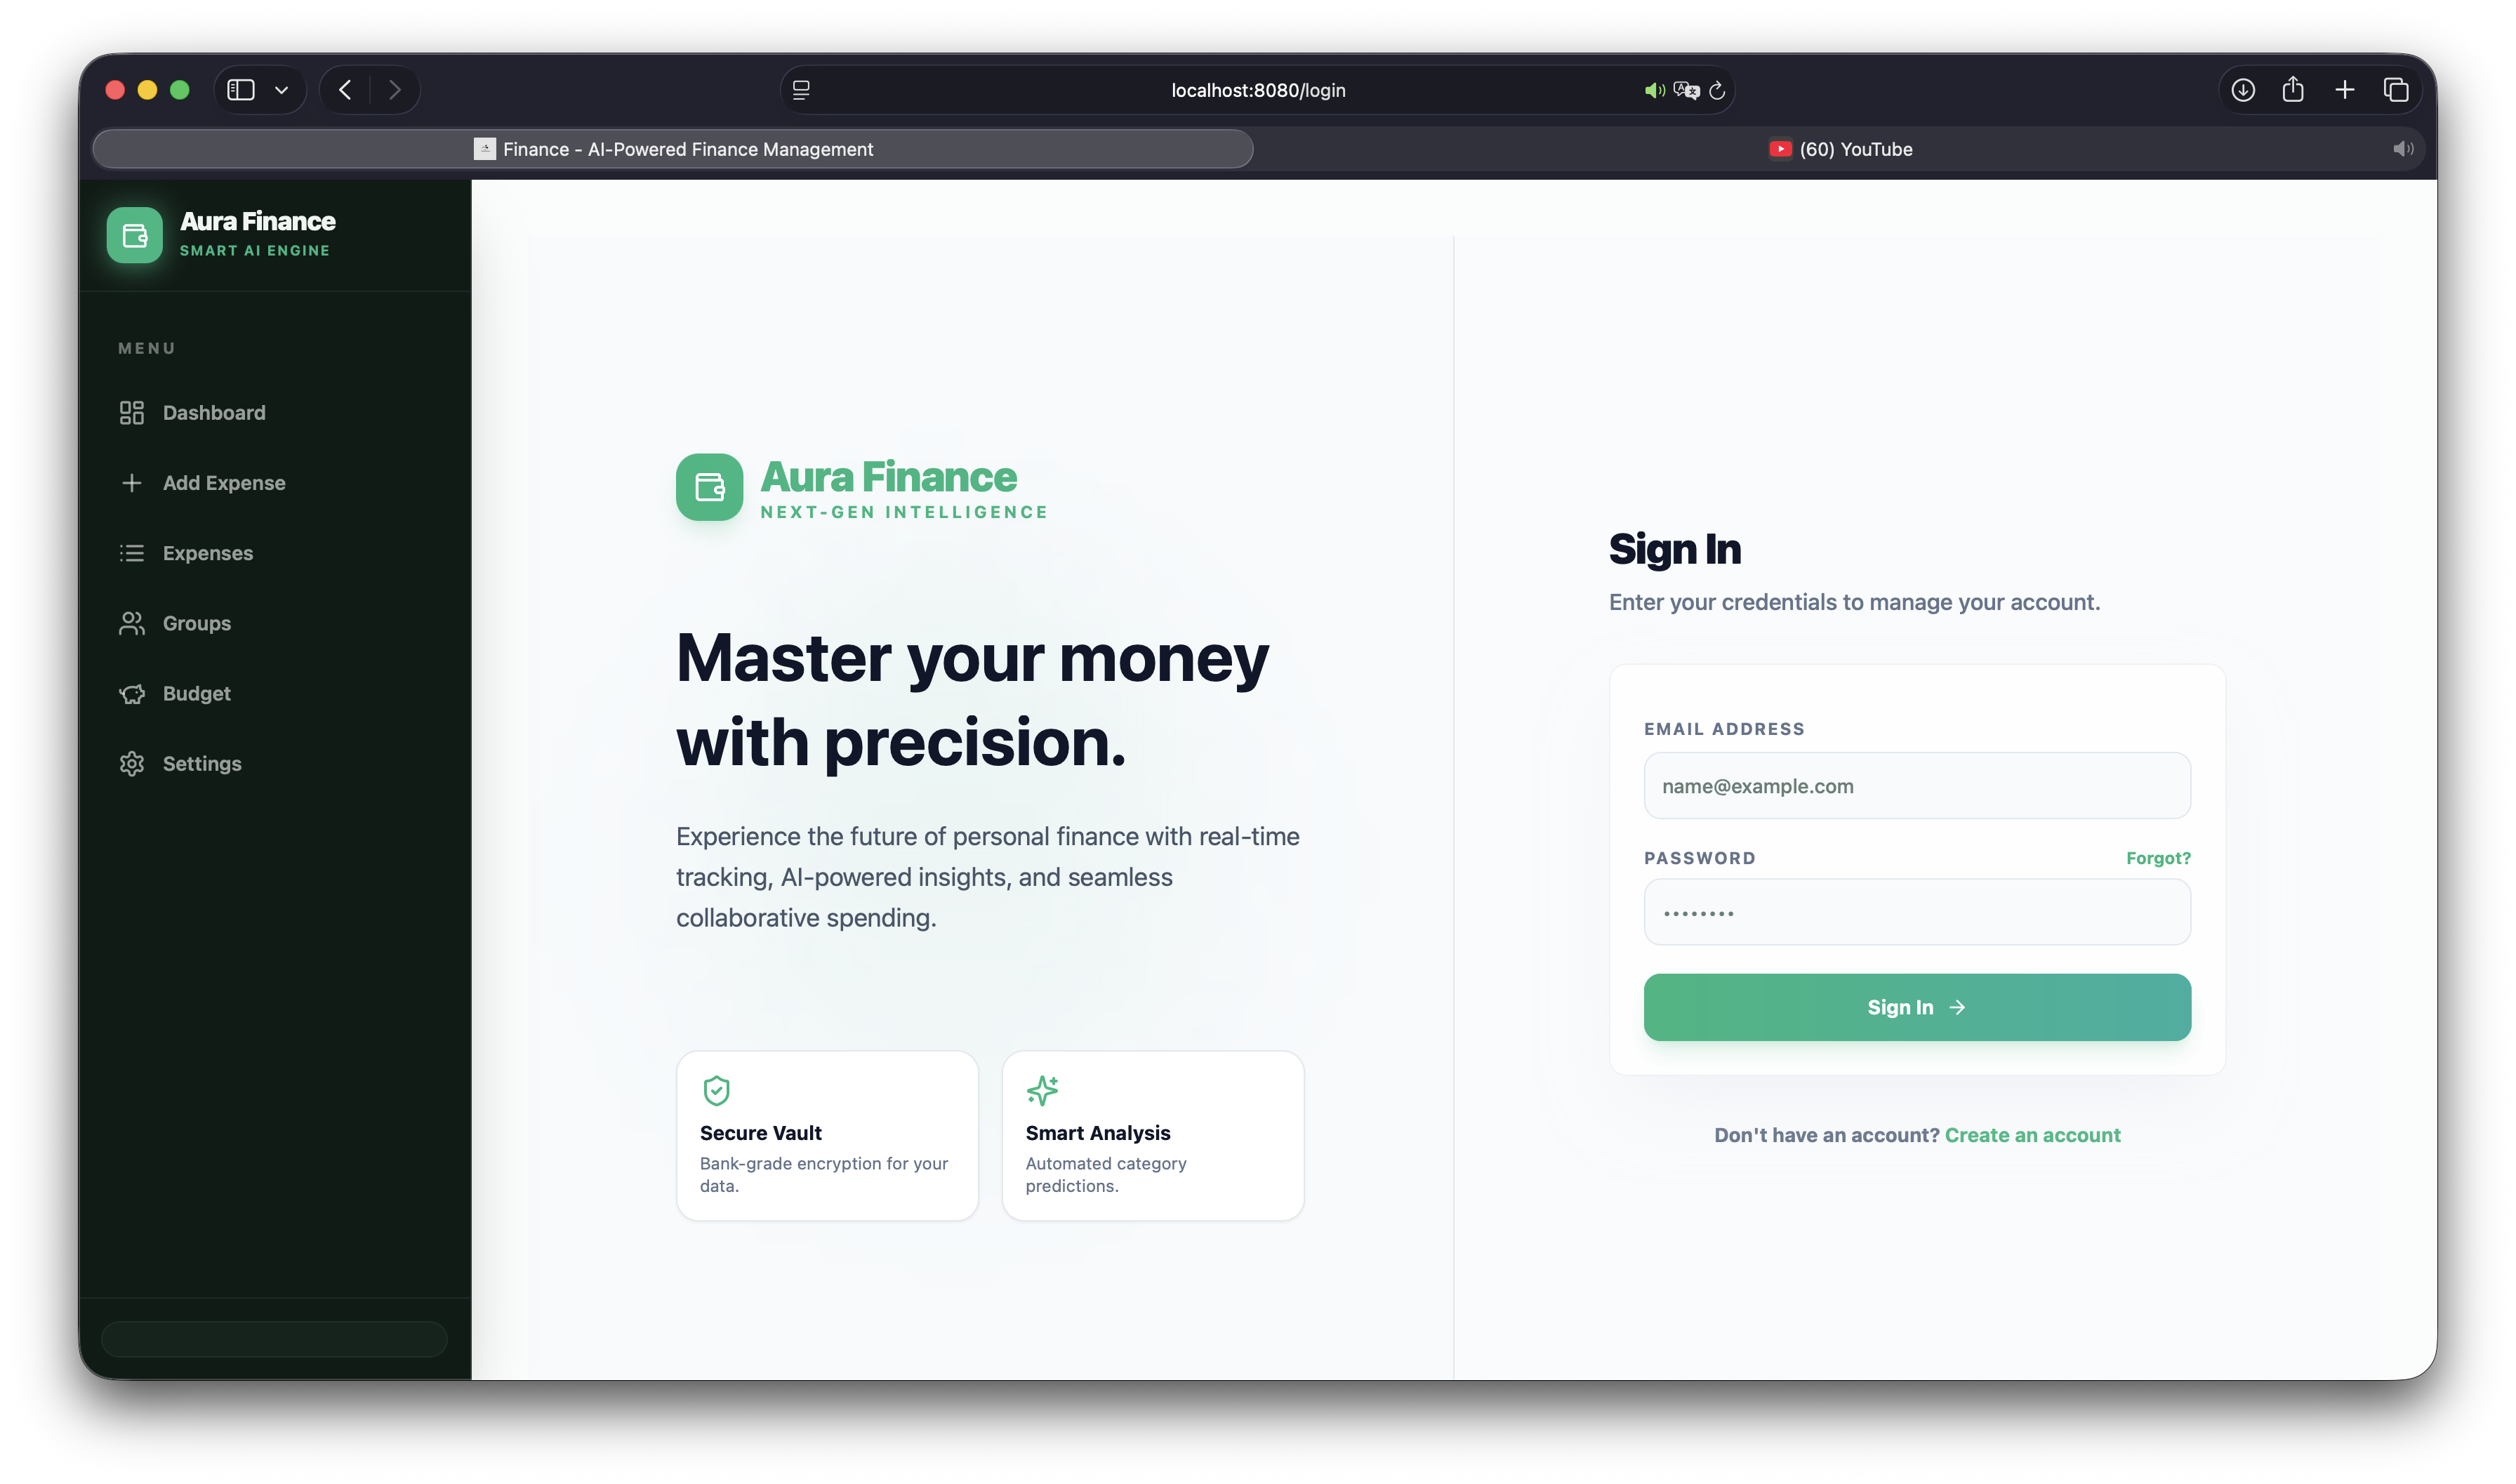
\includegraphics[width=0.8\textwidth]{./fig/aura_sc1}
 \caption{Aura Finance Ana Gösterge Paneli (Dashboard).}
 \label{fig:sc1}
\end{figure}

\begin{figure}[h!]
 \centering
 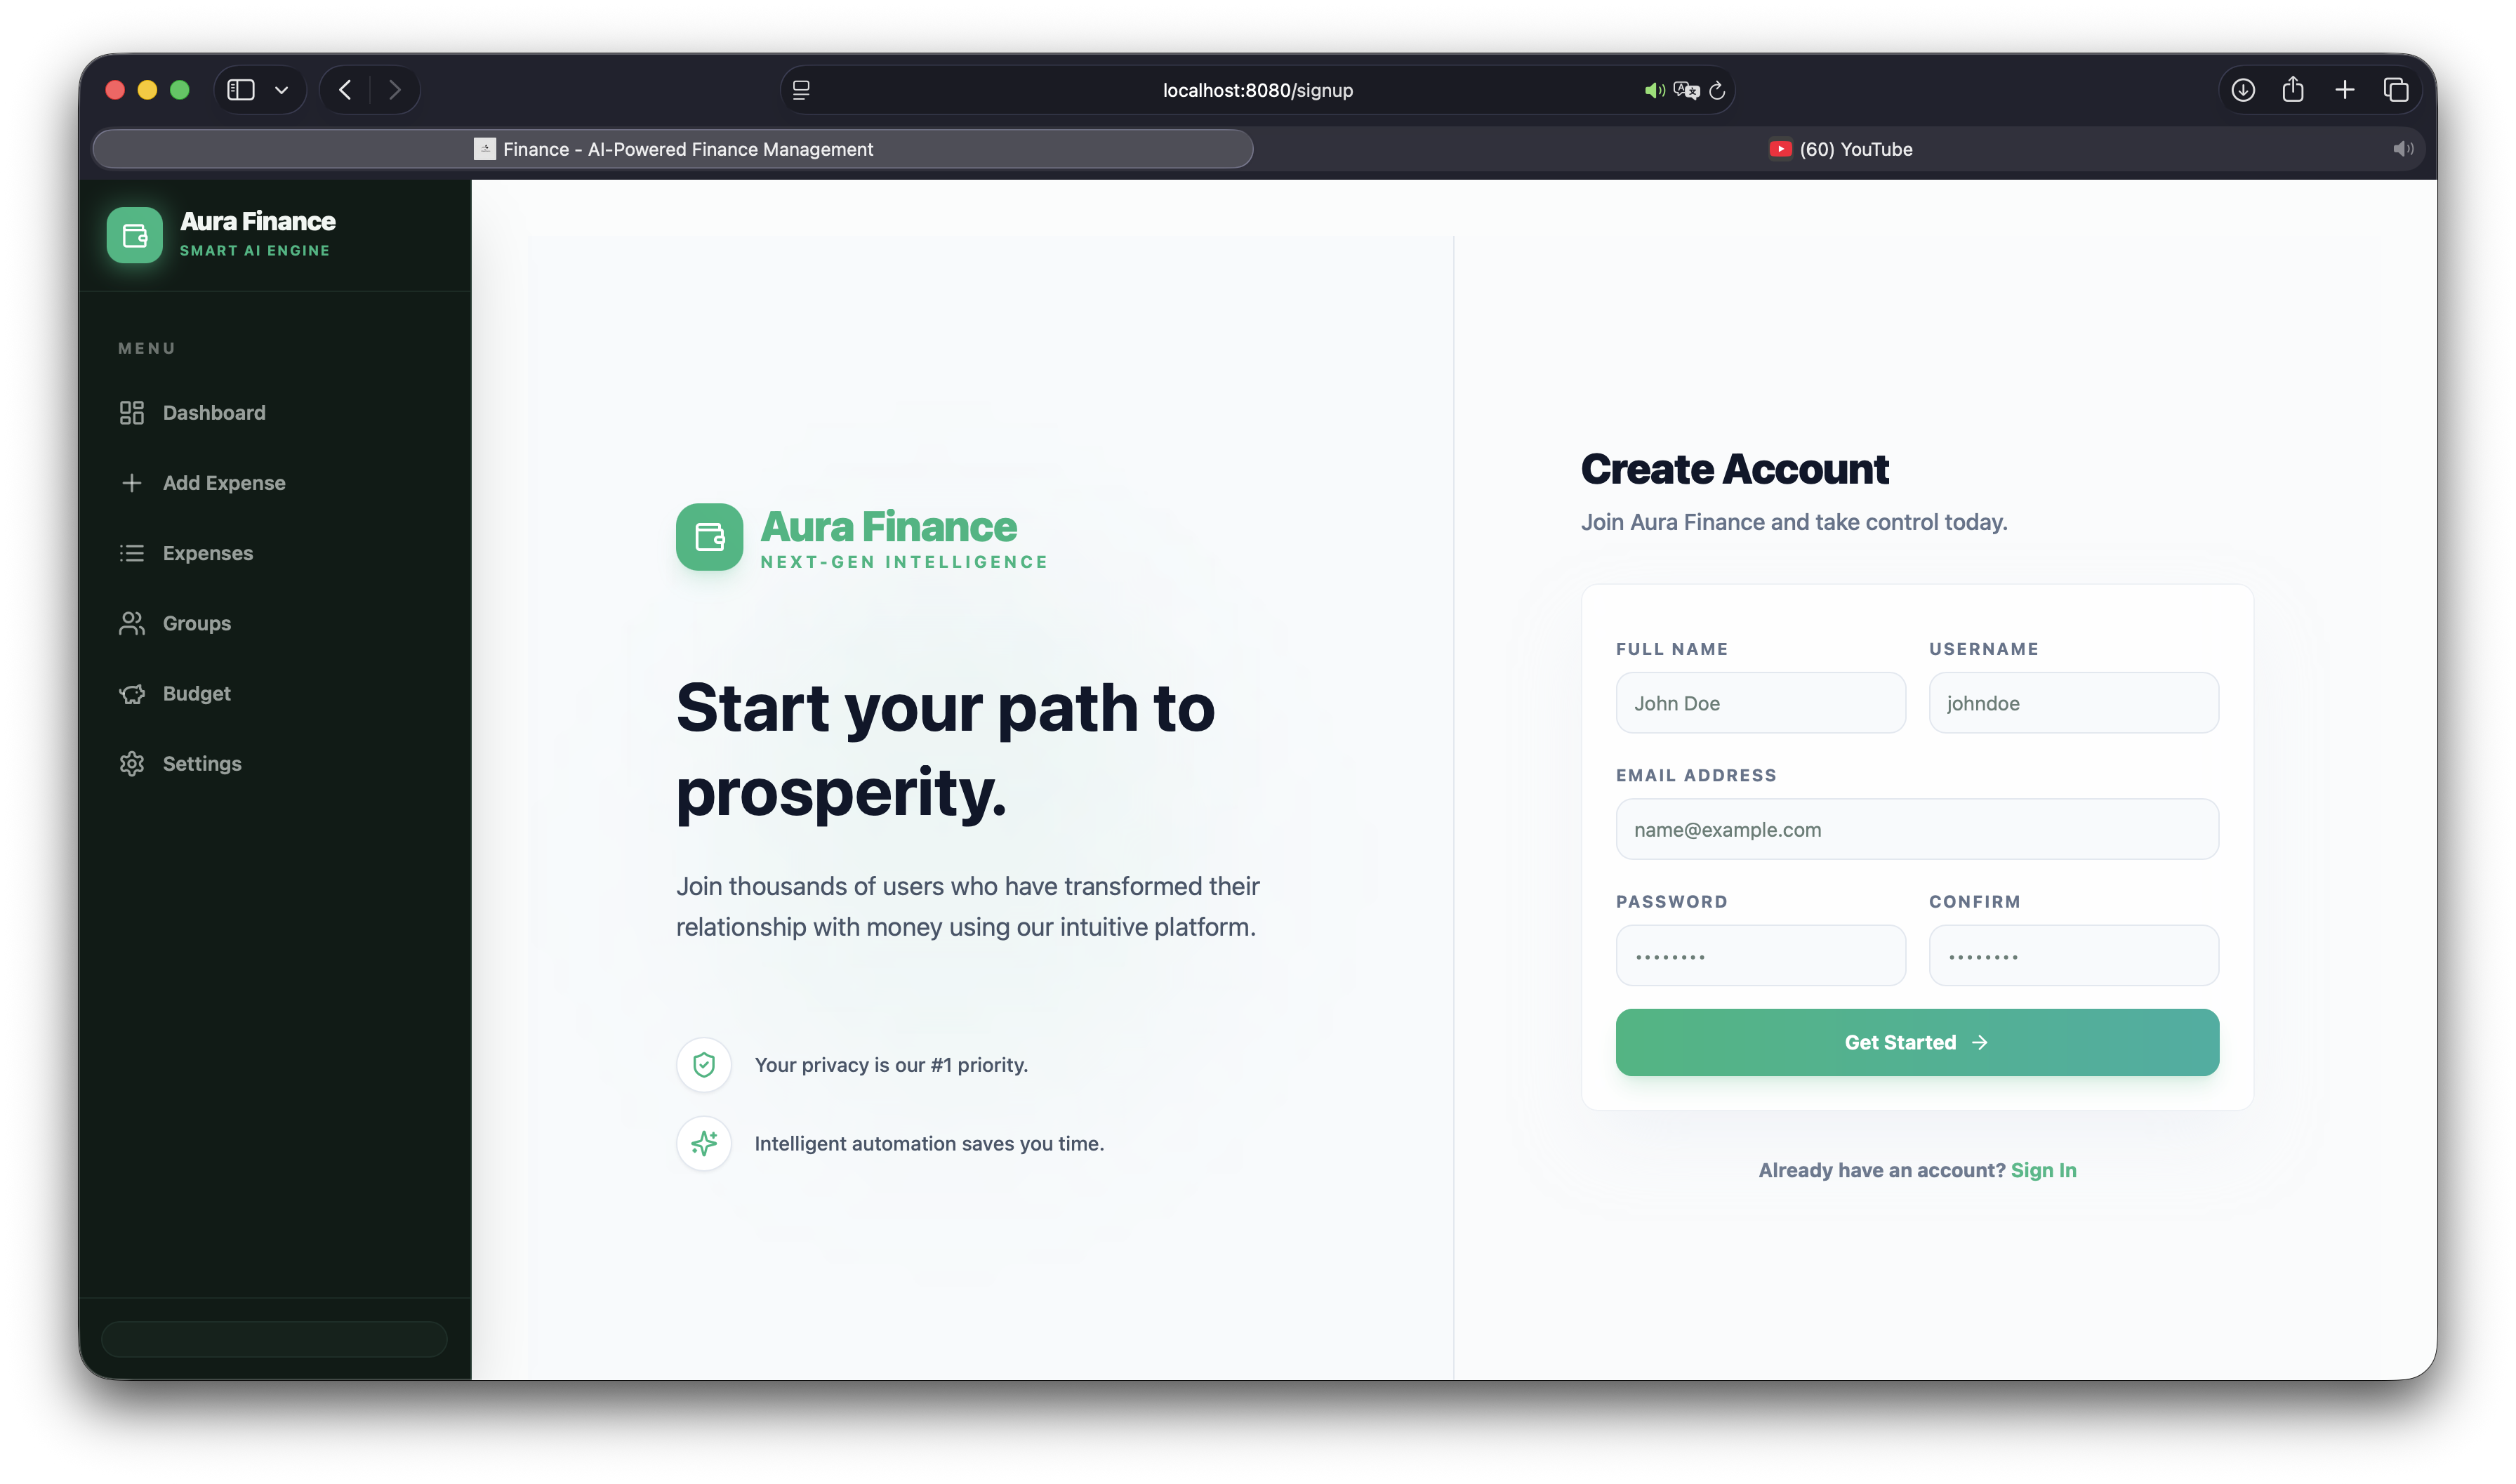
\includegraphics[width=0.8\textwidth]{./fig/aura_sc2}
 \caption{Kullanıcı Harcama Geçmişi ve Analitiği.}
 \label{fig:sc2}
\end{figure}

\begin{figure}[h!]
 \centering
 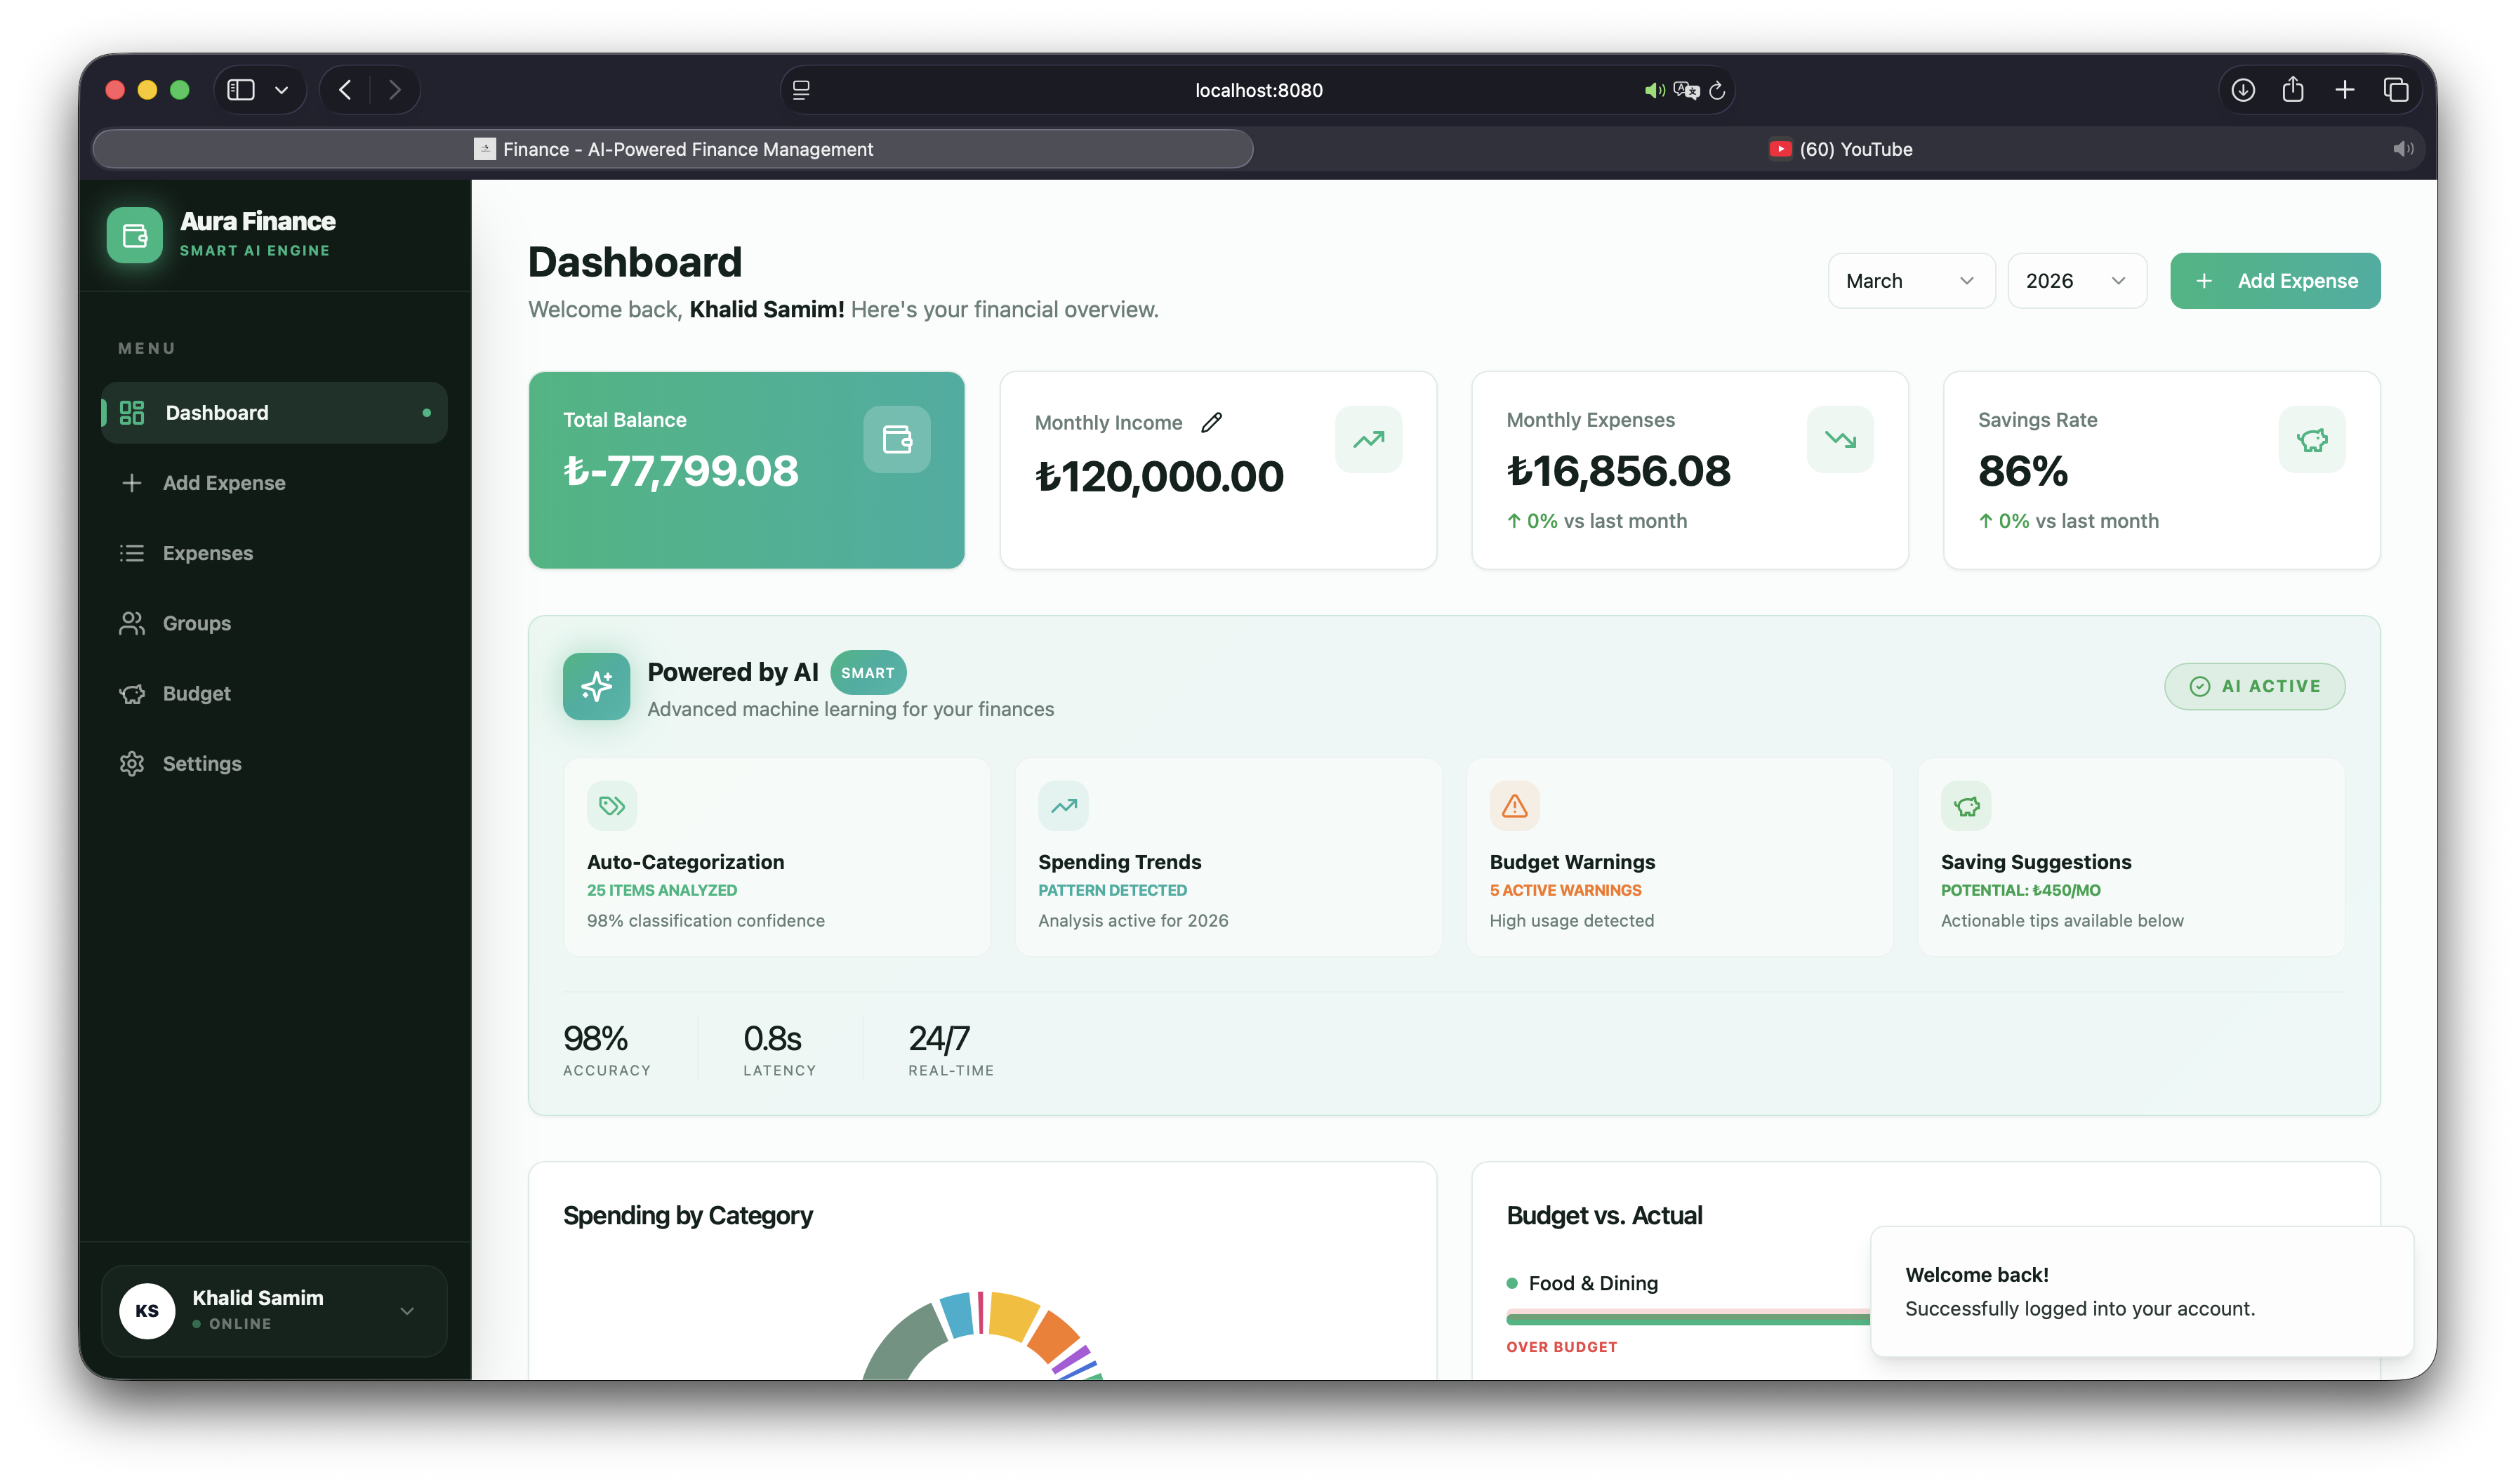
\includegraphics[width=0.8\textwidth]{./fig/aura_sc3}
 \caption{Harcama Filtreleme ve Kategori Bazlı Listeleme.}
 \label{fig:sc3}
\end{figure}

\section{Yapay Zekâ ve Tahminleme Bulguları}

Uygulamanın yapay zekâ modülleri, kullanıcıların finansal sağlığını korumak adına proaktif çözümler sunmaktadır.

\begin{figure}[h!]
 \centering
 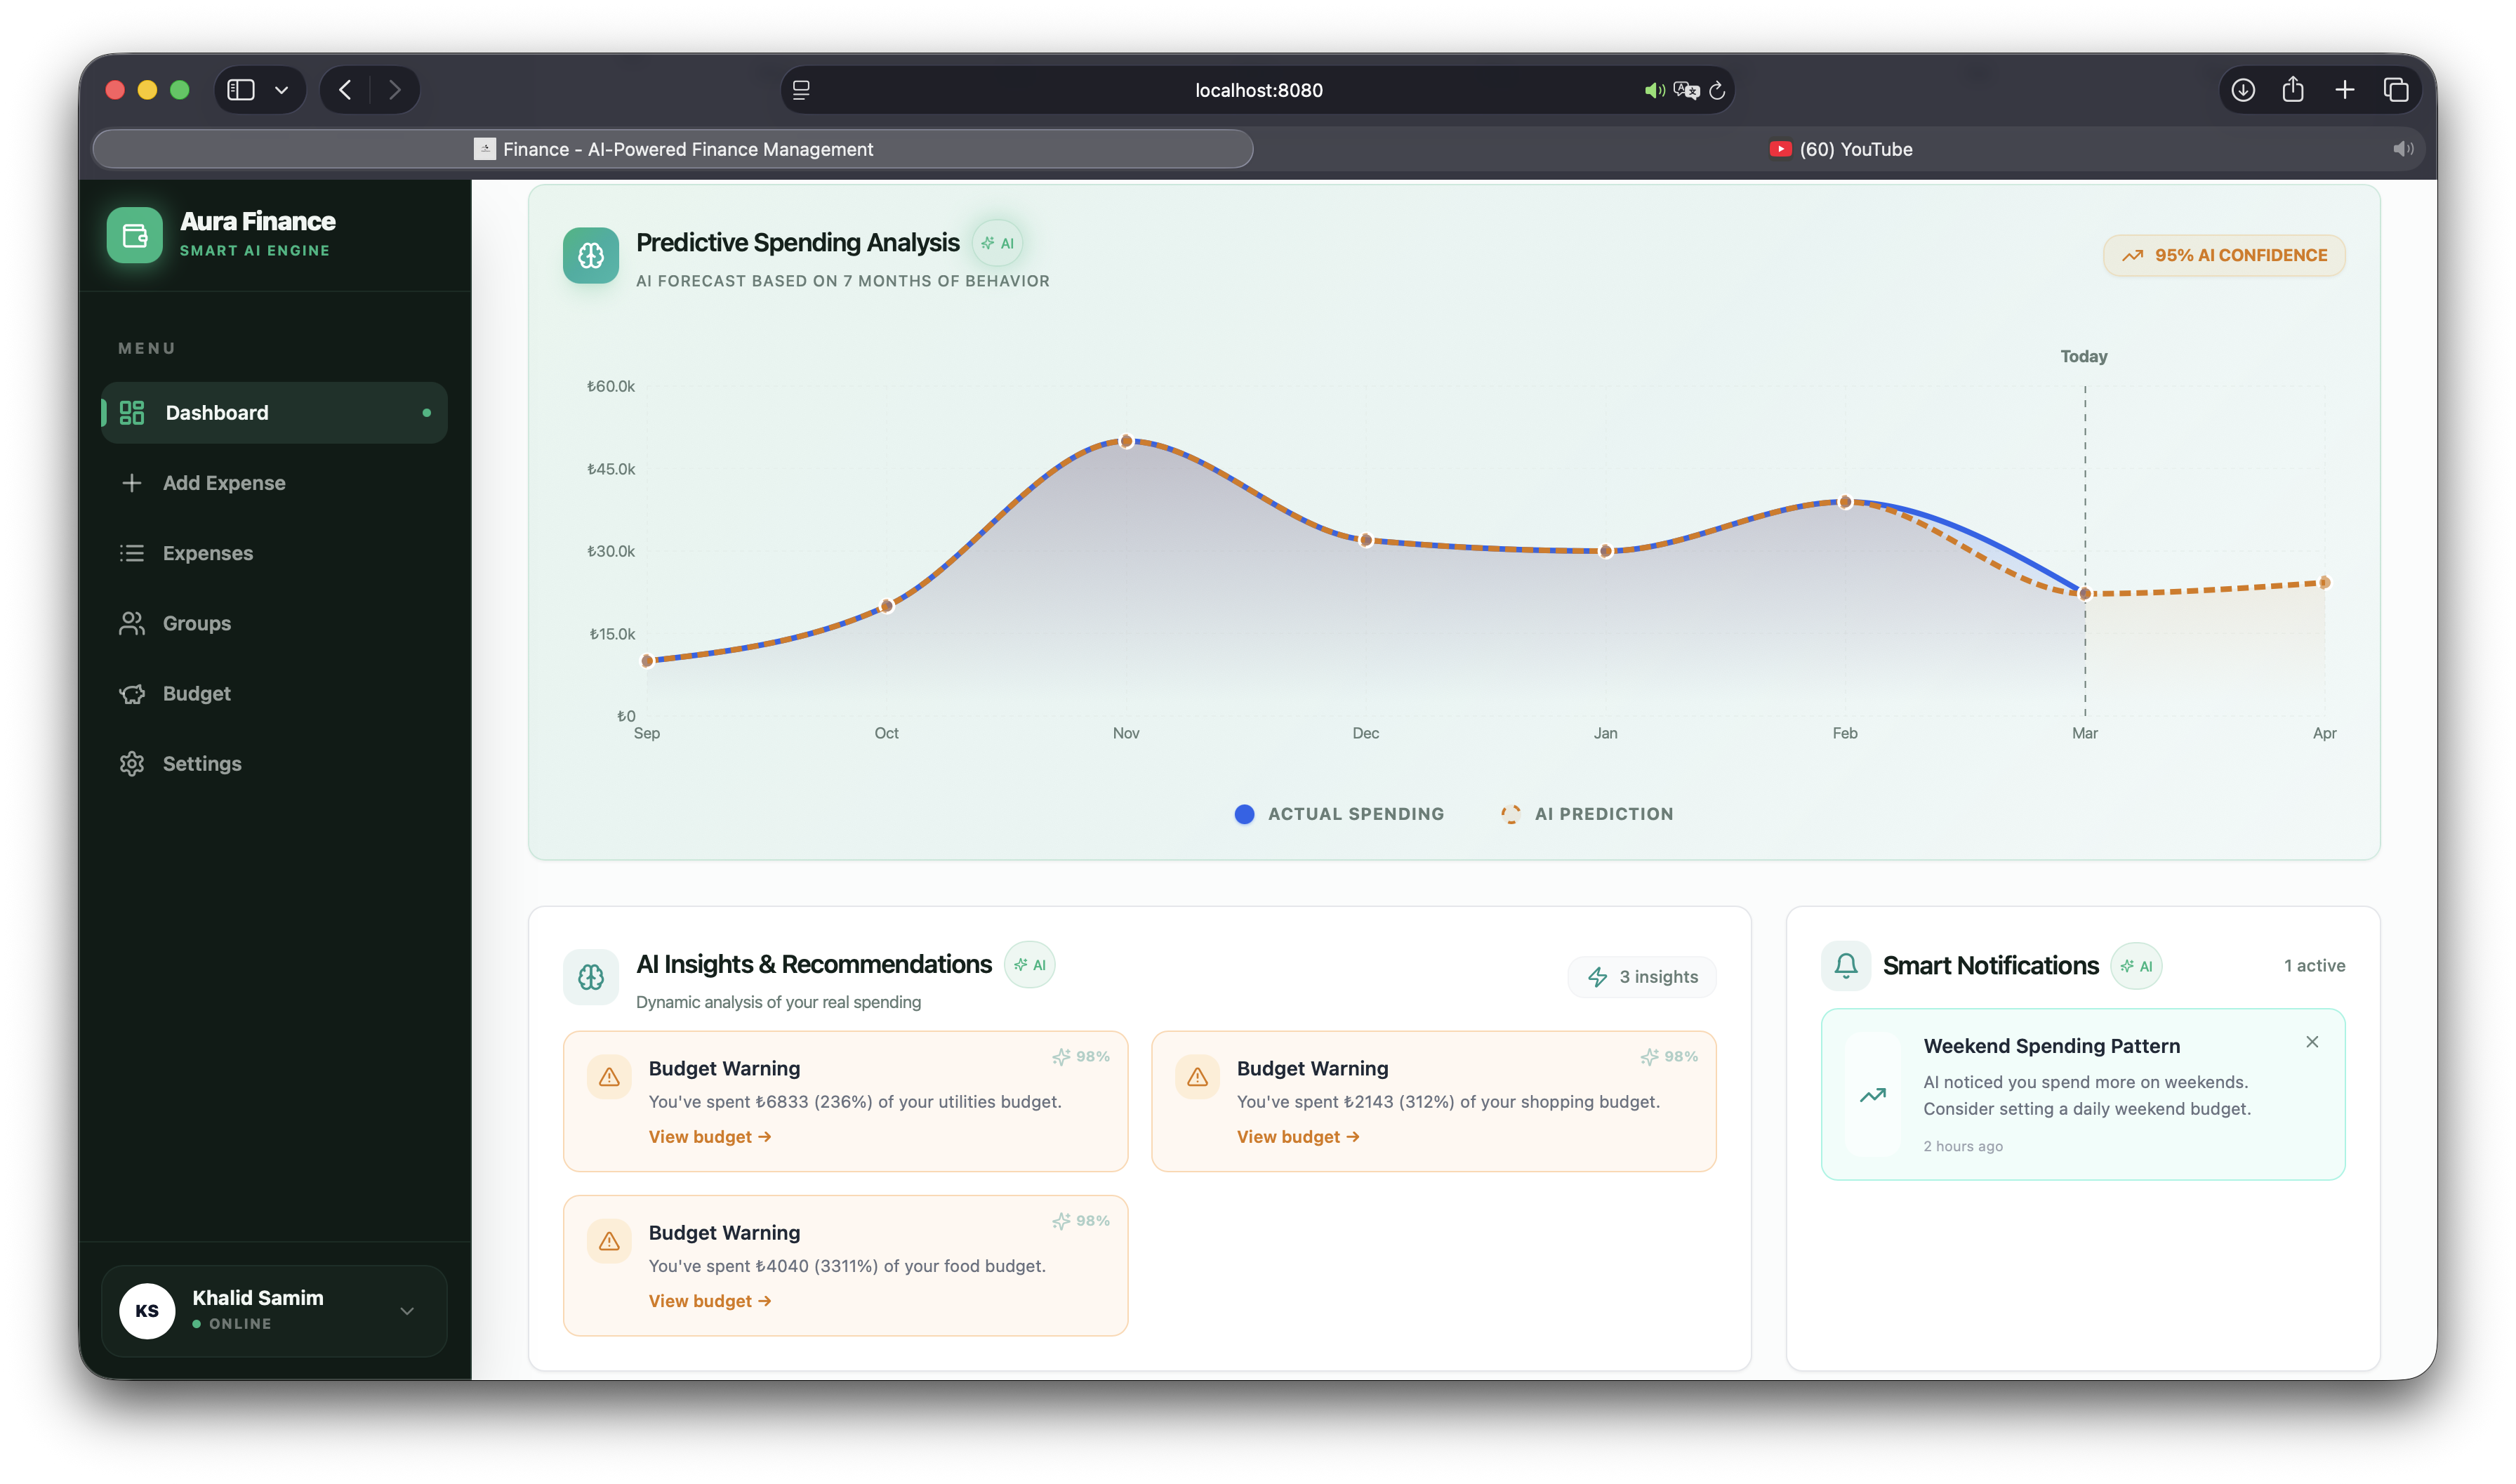
\includegraphics[width=0.8\textwidth]{./fig/aura_sc4}
 \caption{AI Insights: Otomatik Harcama Analizi ve Bildirimler.}
 \label{fig:sc4}
\end{figure}

\begin{figure}[h!]
 \centering
 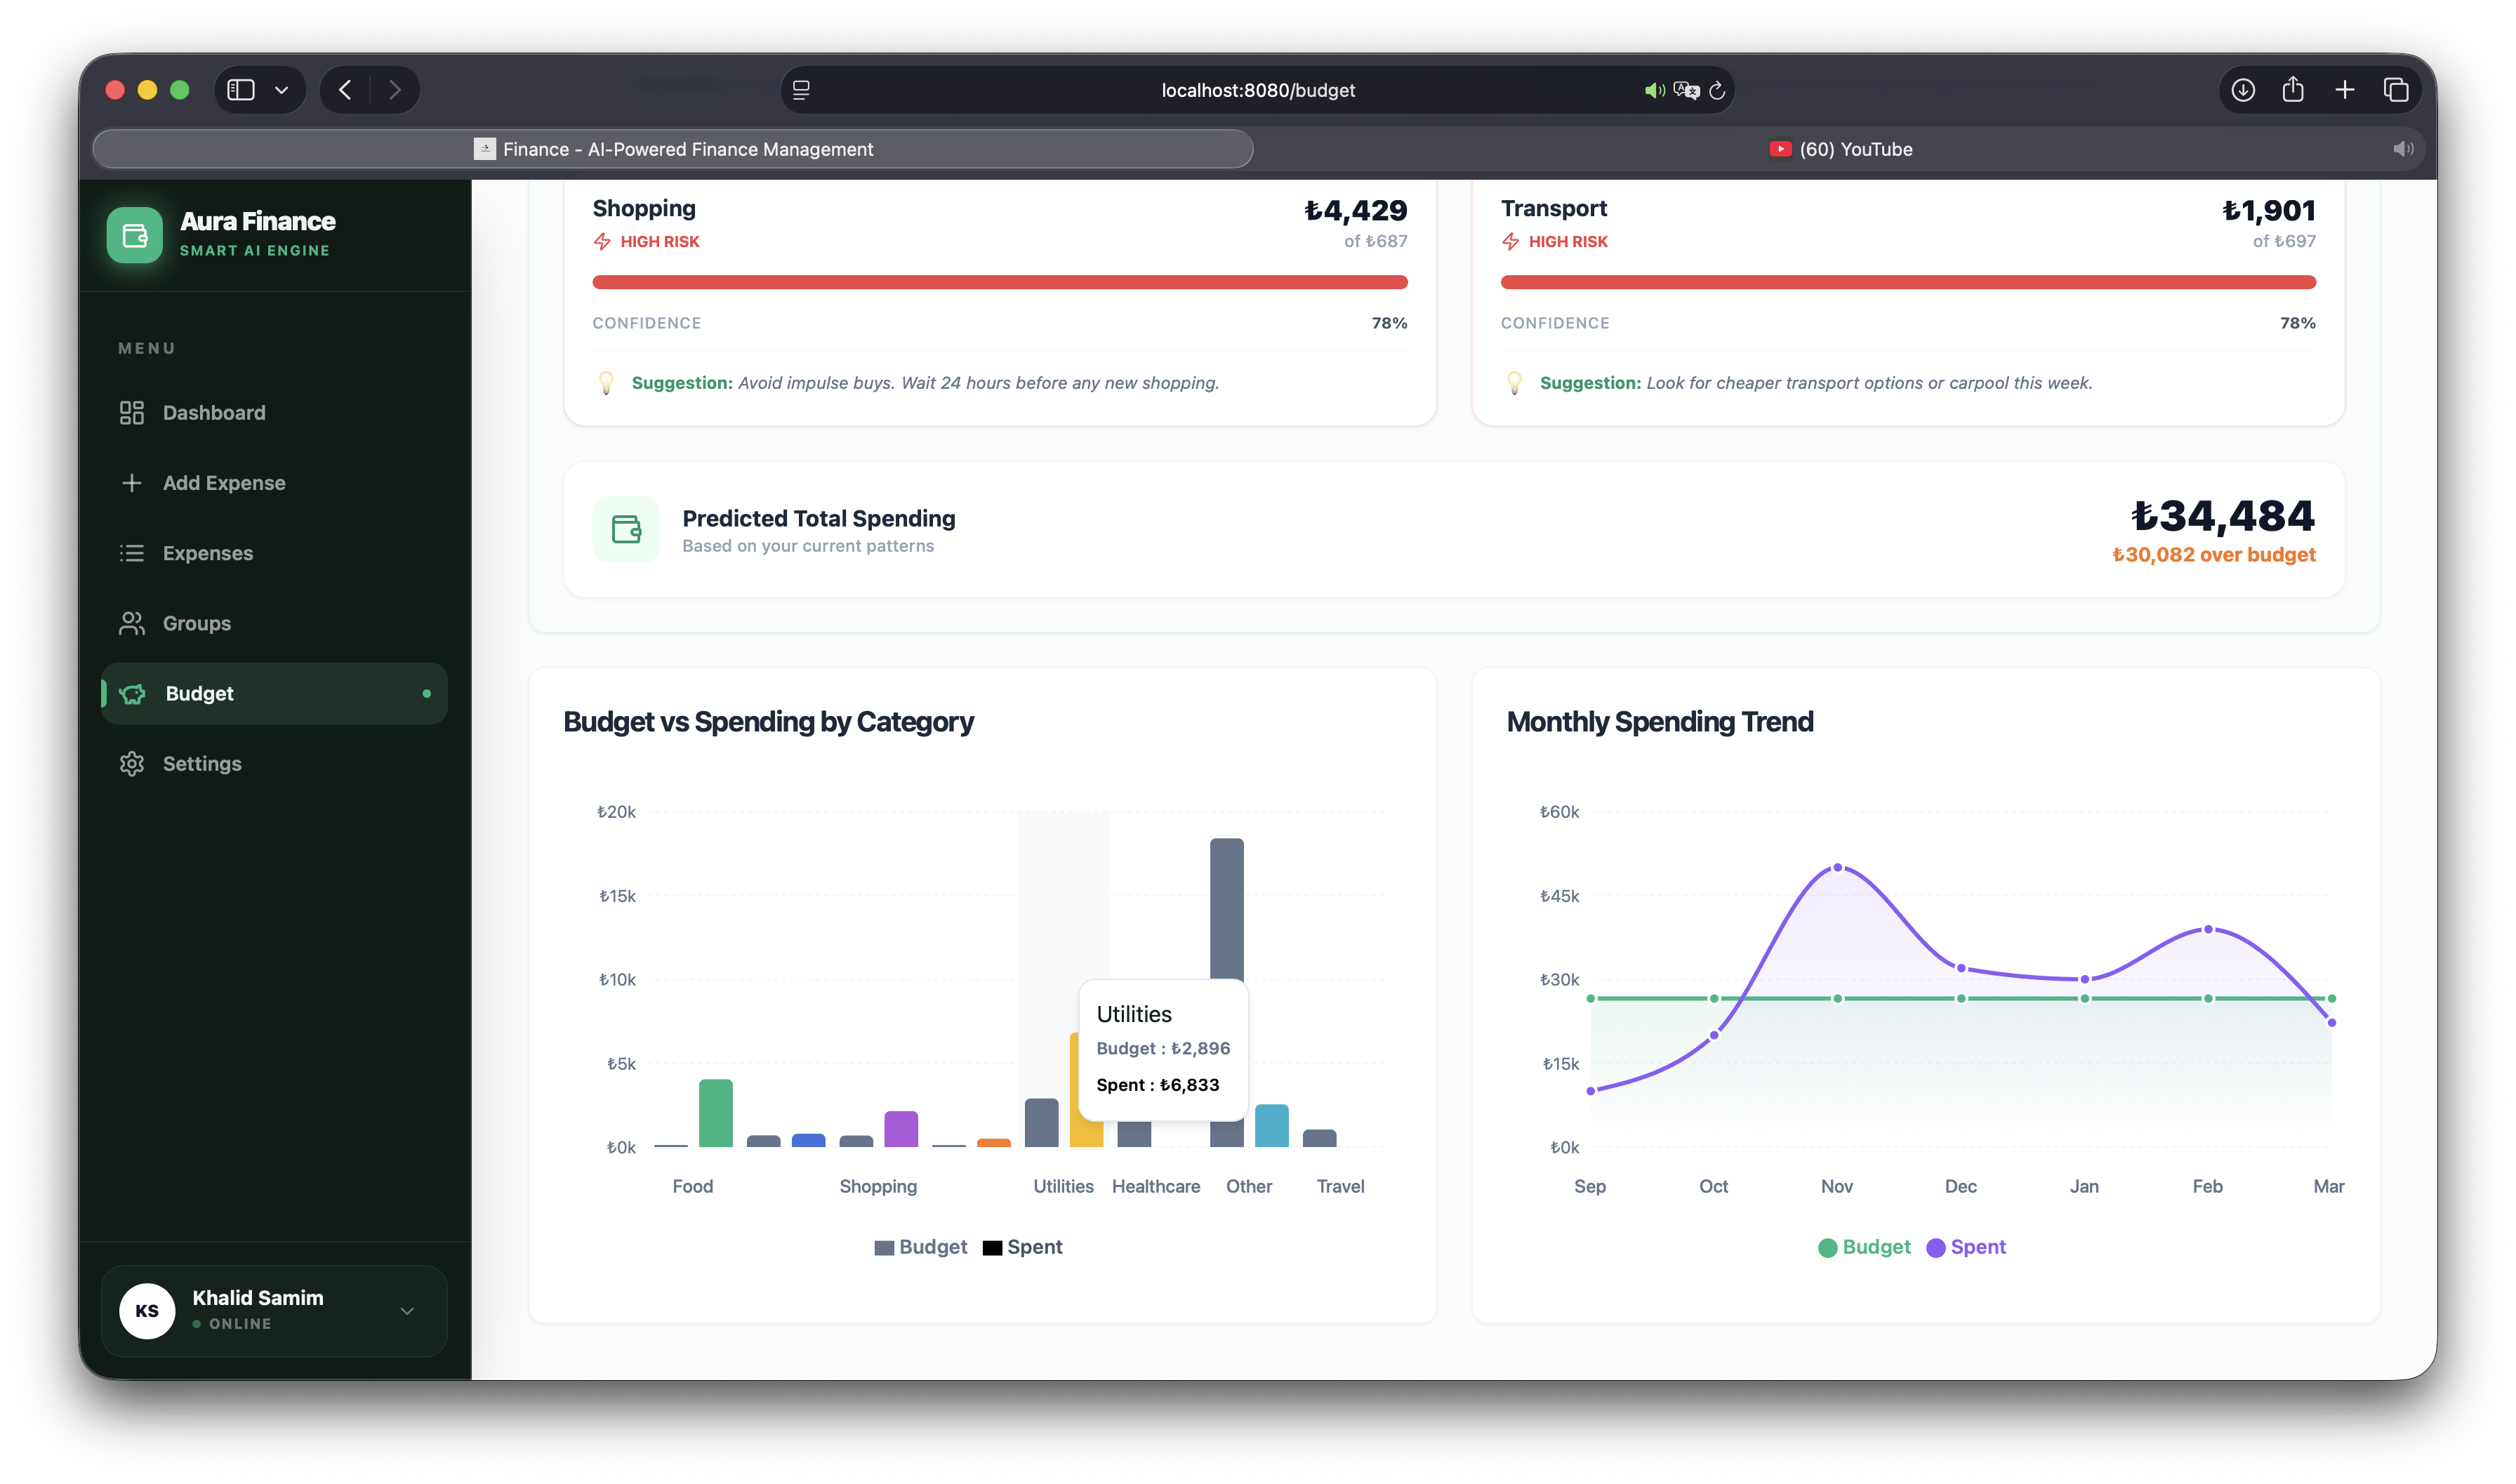
\includegraphics[width=0.8\textwidth]{./fig/aura_sc9}
 \caption{Hibrit Bütçe Optimizasyon Önerileri.}
 \label{fig:sc9}
\end{figure}

\begin{figure}[h!]
 \centering
 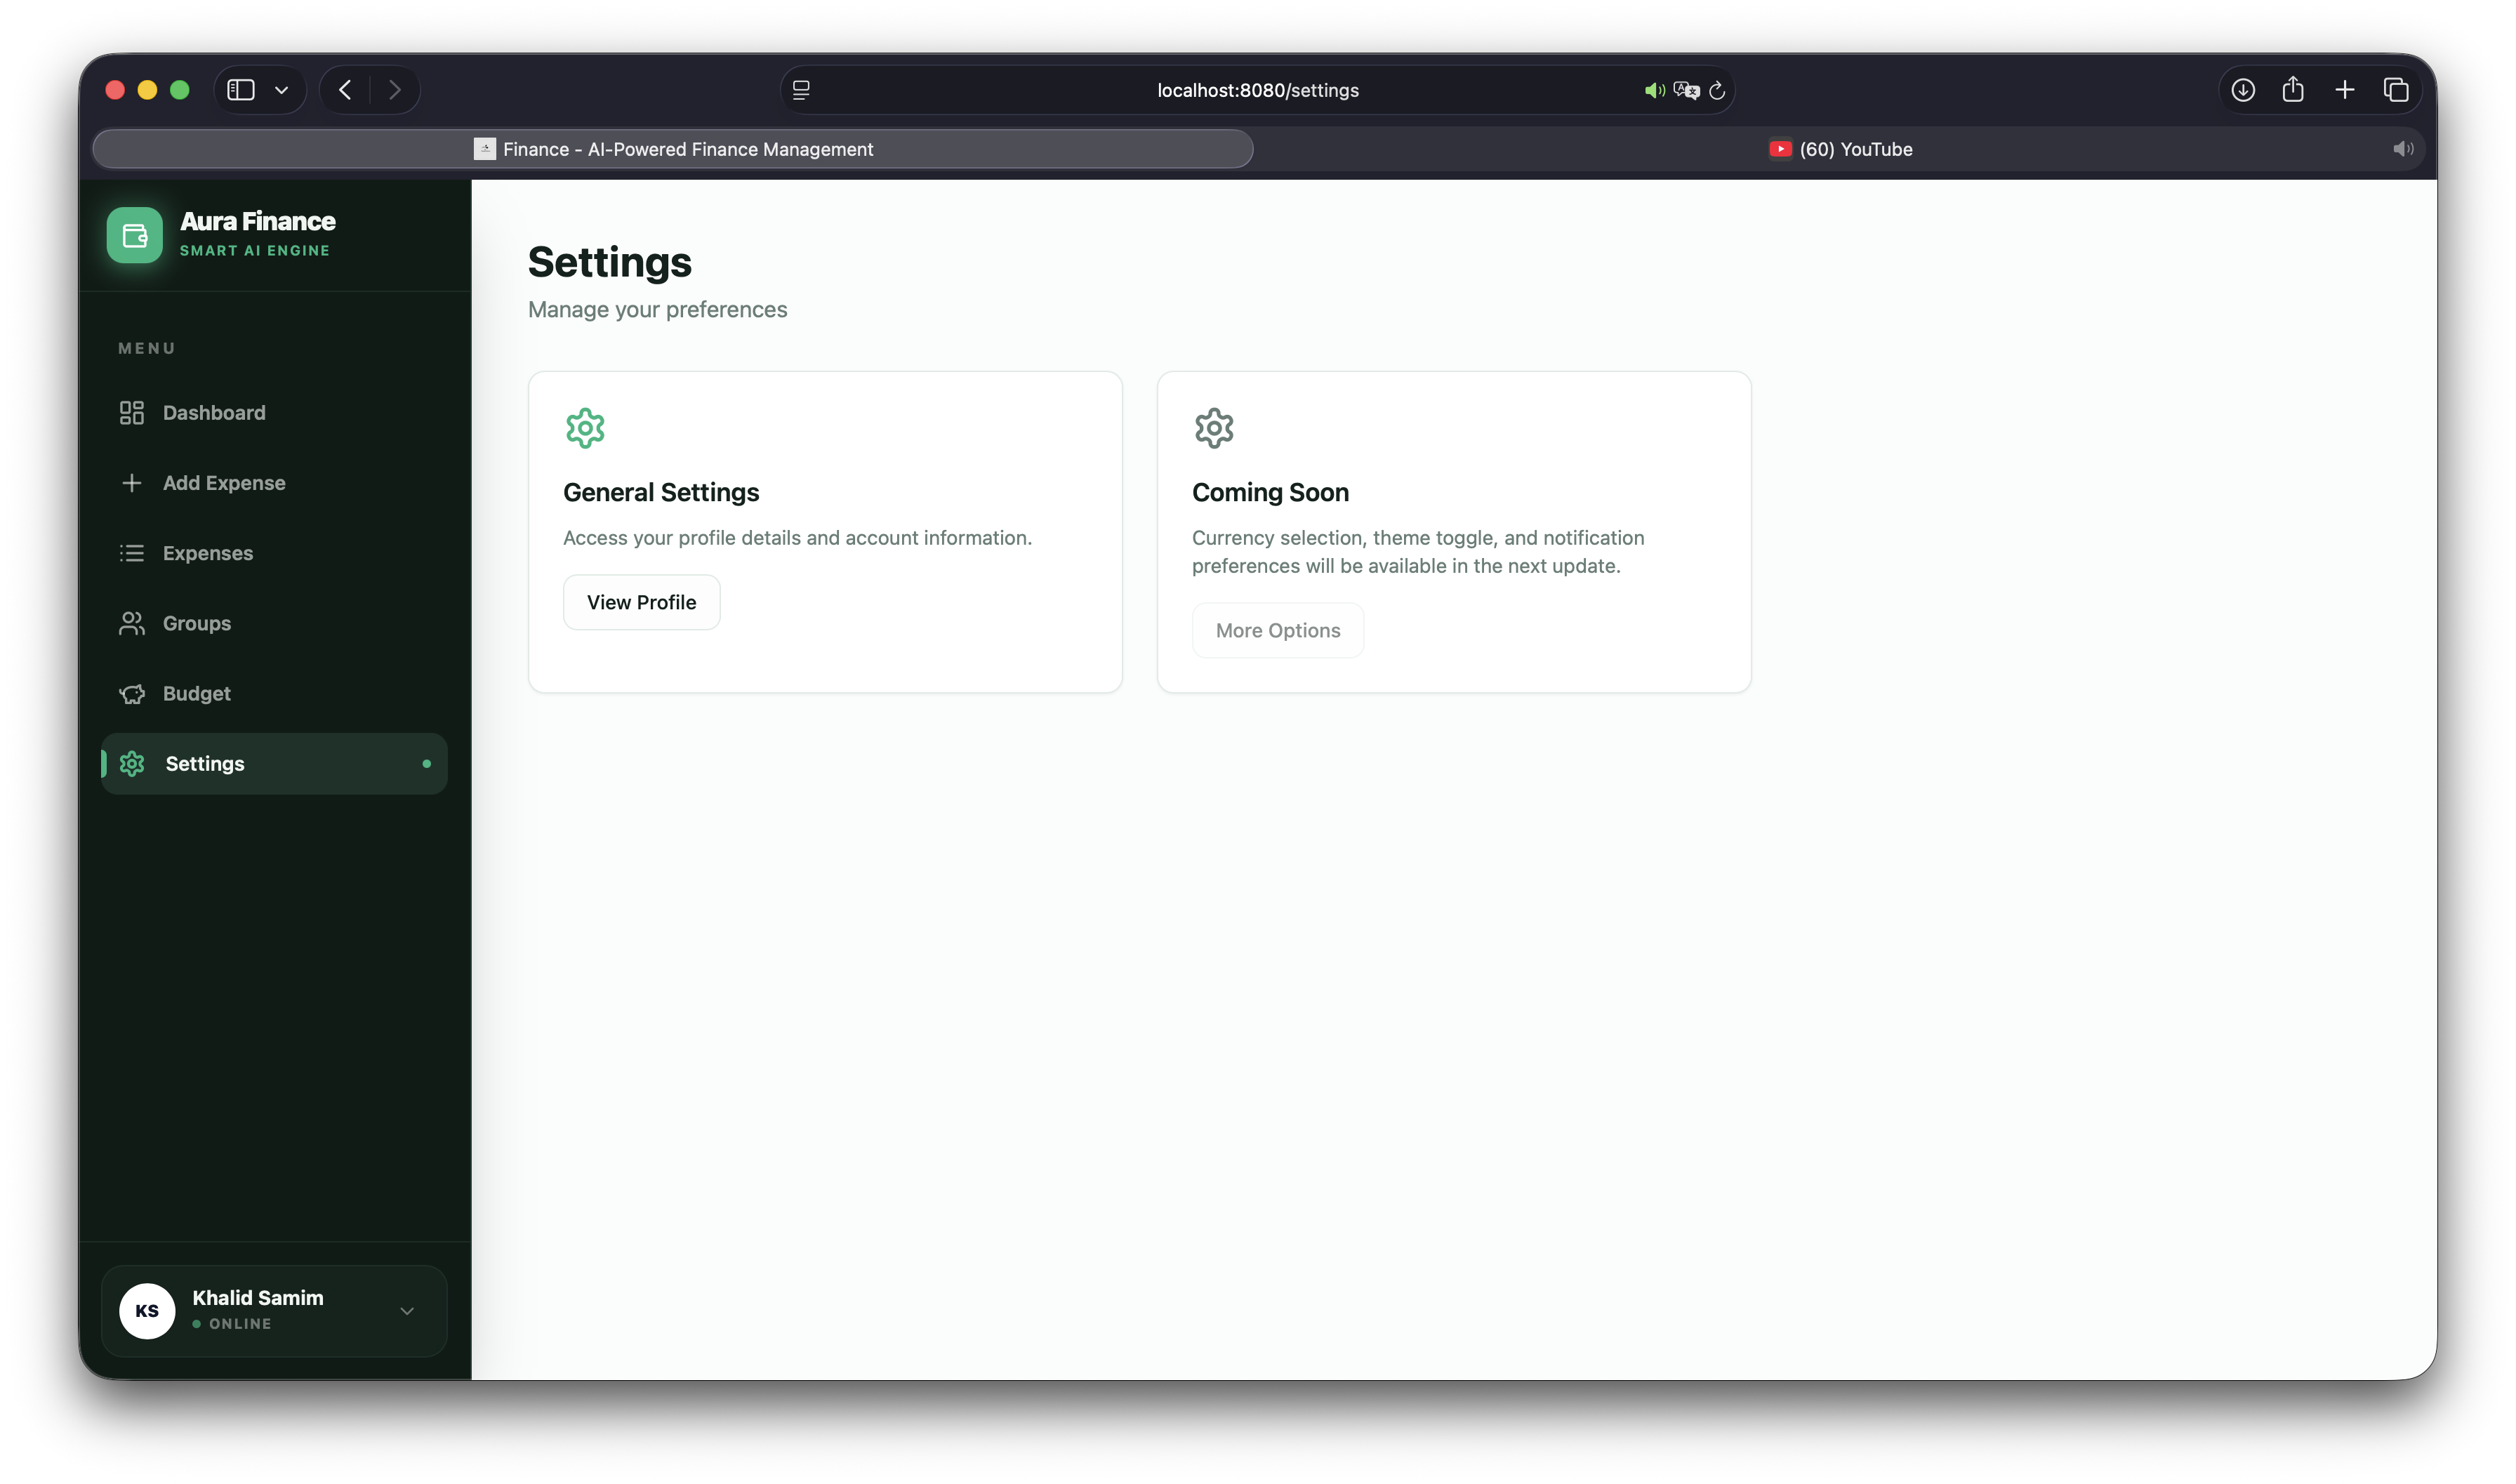
\includegraphics[width=0.8\textwidth]{./fig/aura_sc10}
 \caption{LSTM Tabanlı Gelecek Ay Harcama Tahmin Grafiği.}
 \label{fig:sc10}
\end{figure}

\section{Akıllı Veri Giriş Yöntemleri ve Gruplar}

OCR ve sesli komut teknolojileri, veri giriş sürecini otomatize ederek kullanıcı yükünü azaltmaktadır.

\begin{figure}[h!]
 \centering
 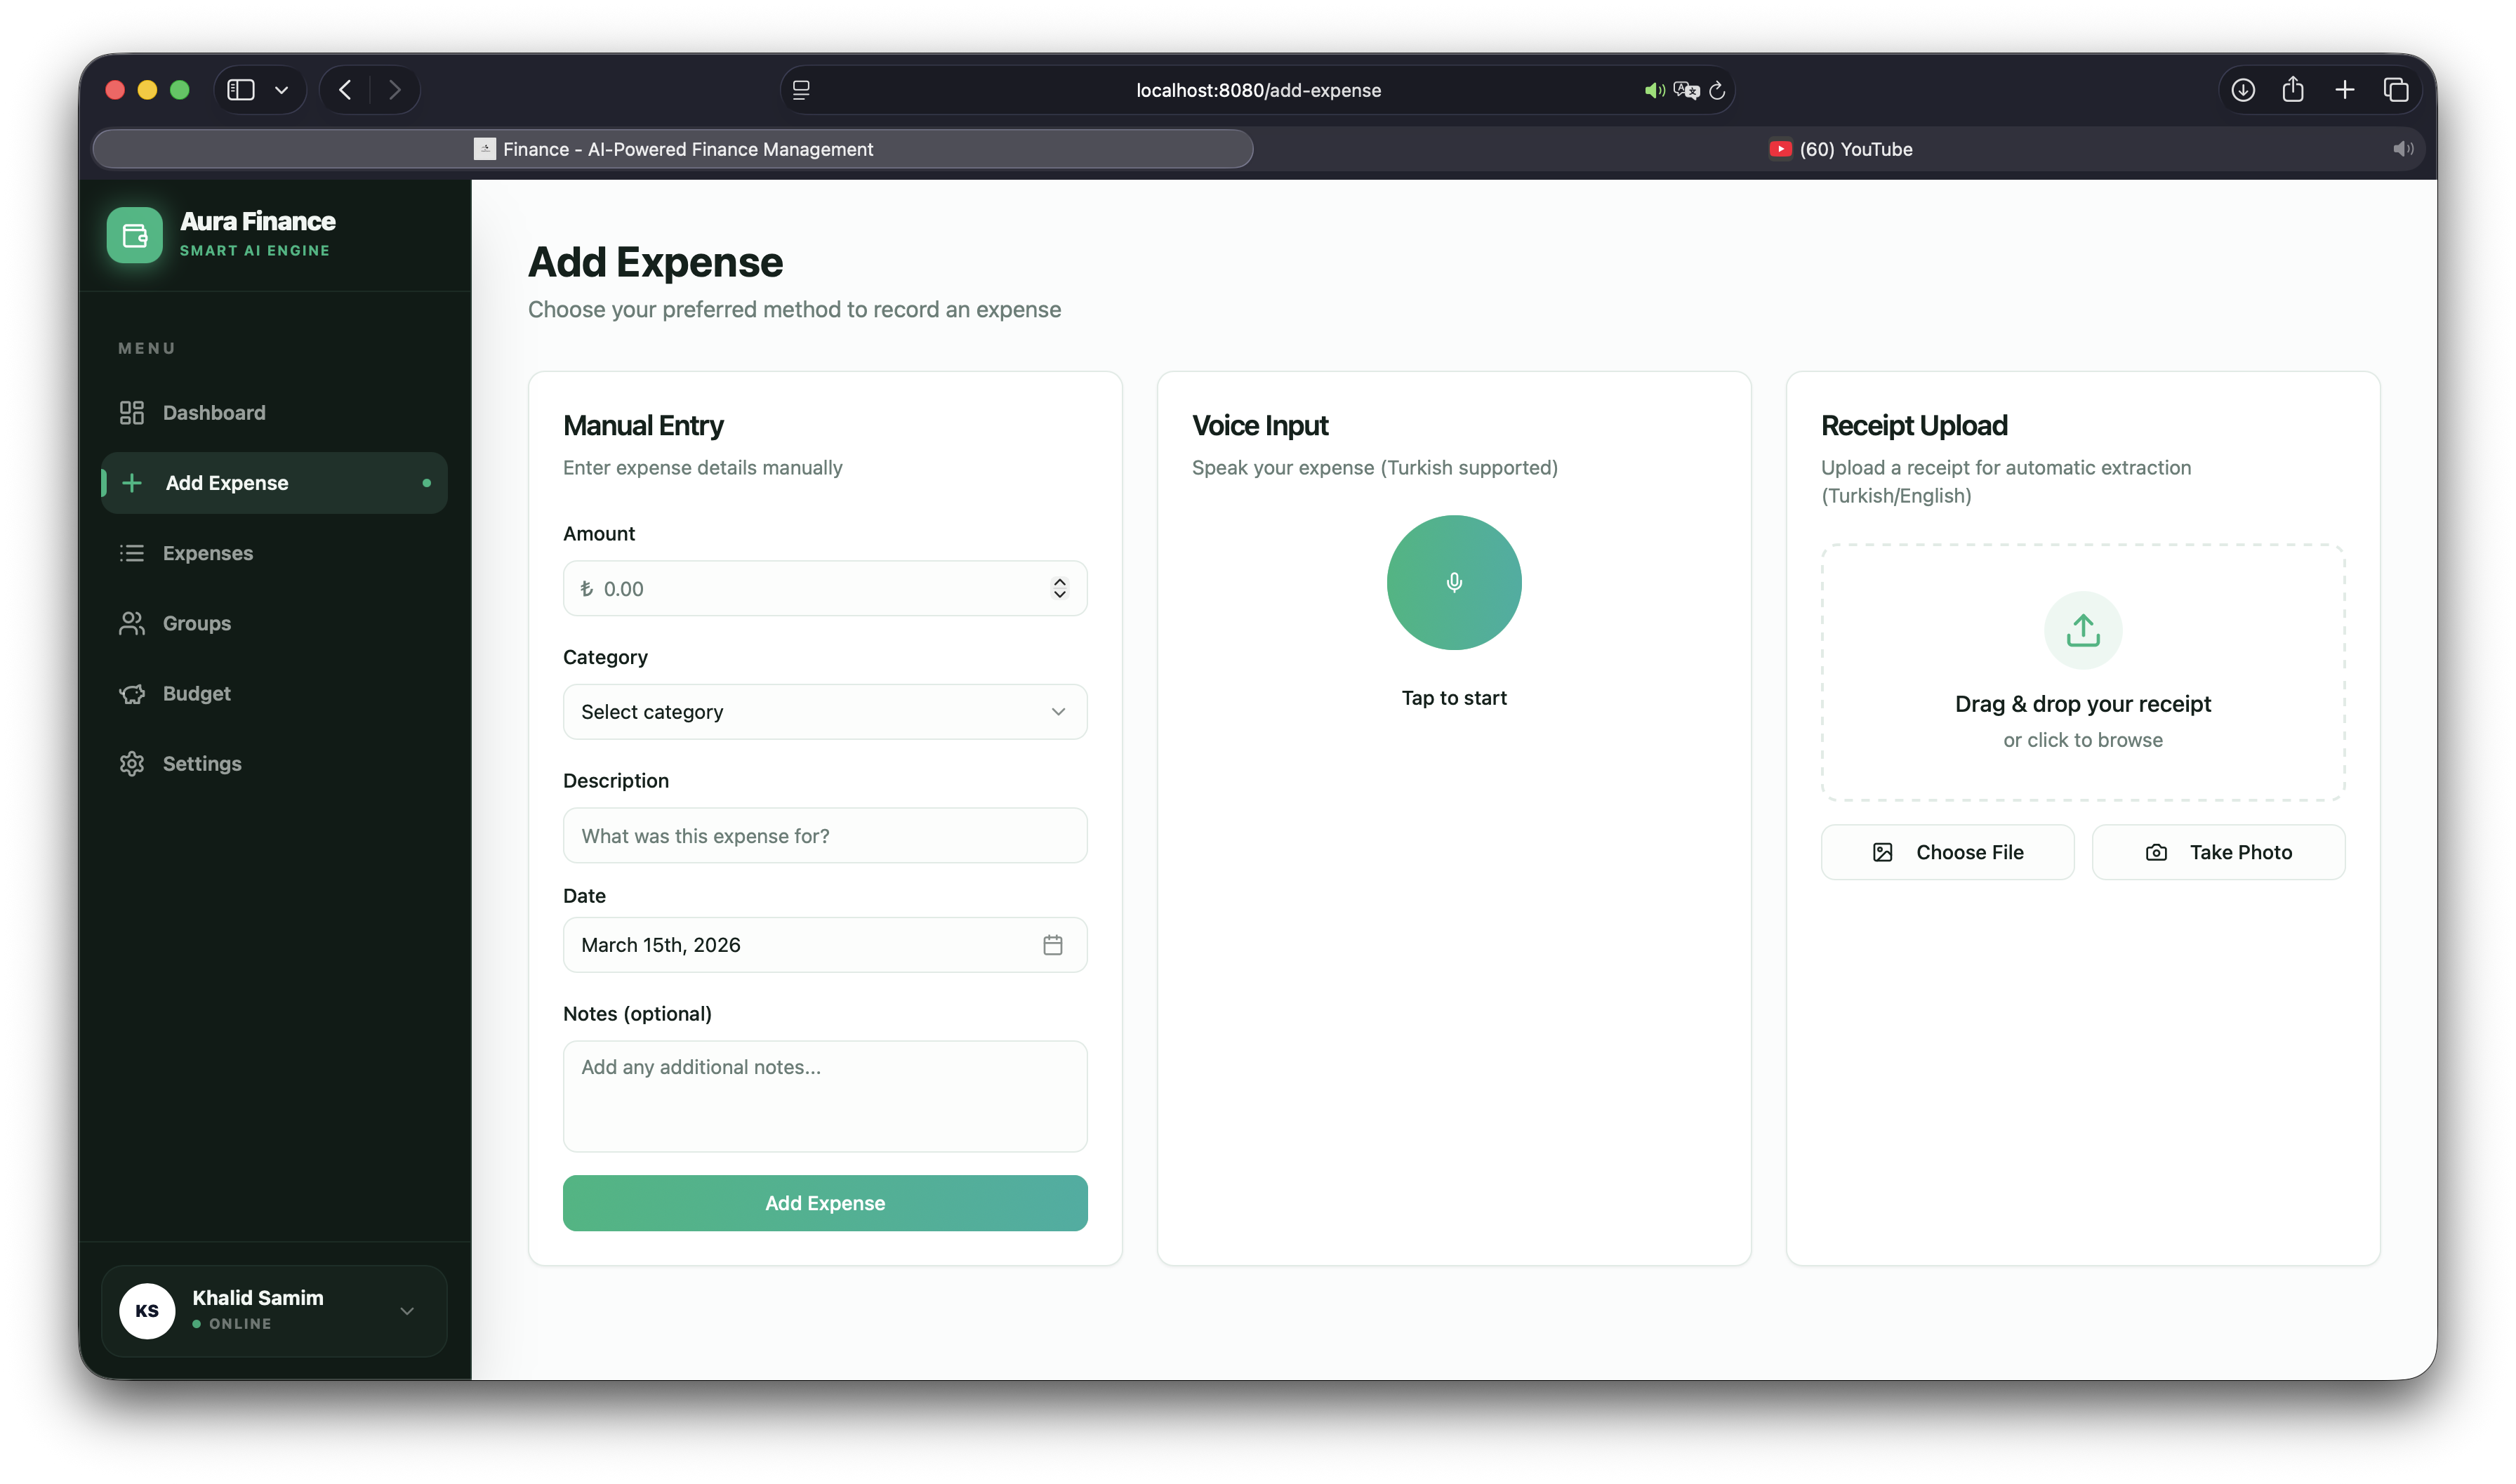
\includegraphics[width=0.6\textwidth]{./fig/aura_sc5}
 \caption{OCR ile Otomatik Makbuz Okuma ve Veri Ayrıştırma.}
 \label{fig:sc5}
\end{figure}

\begin{figure}[h!]
 \centering
 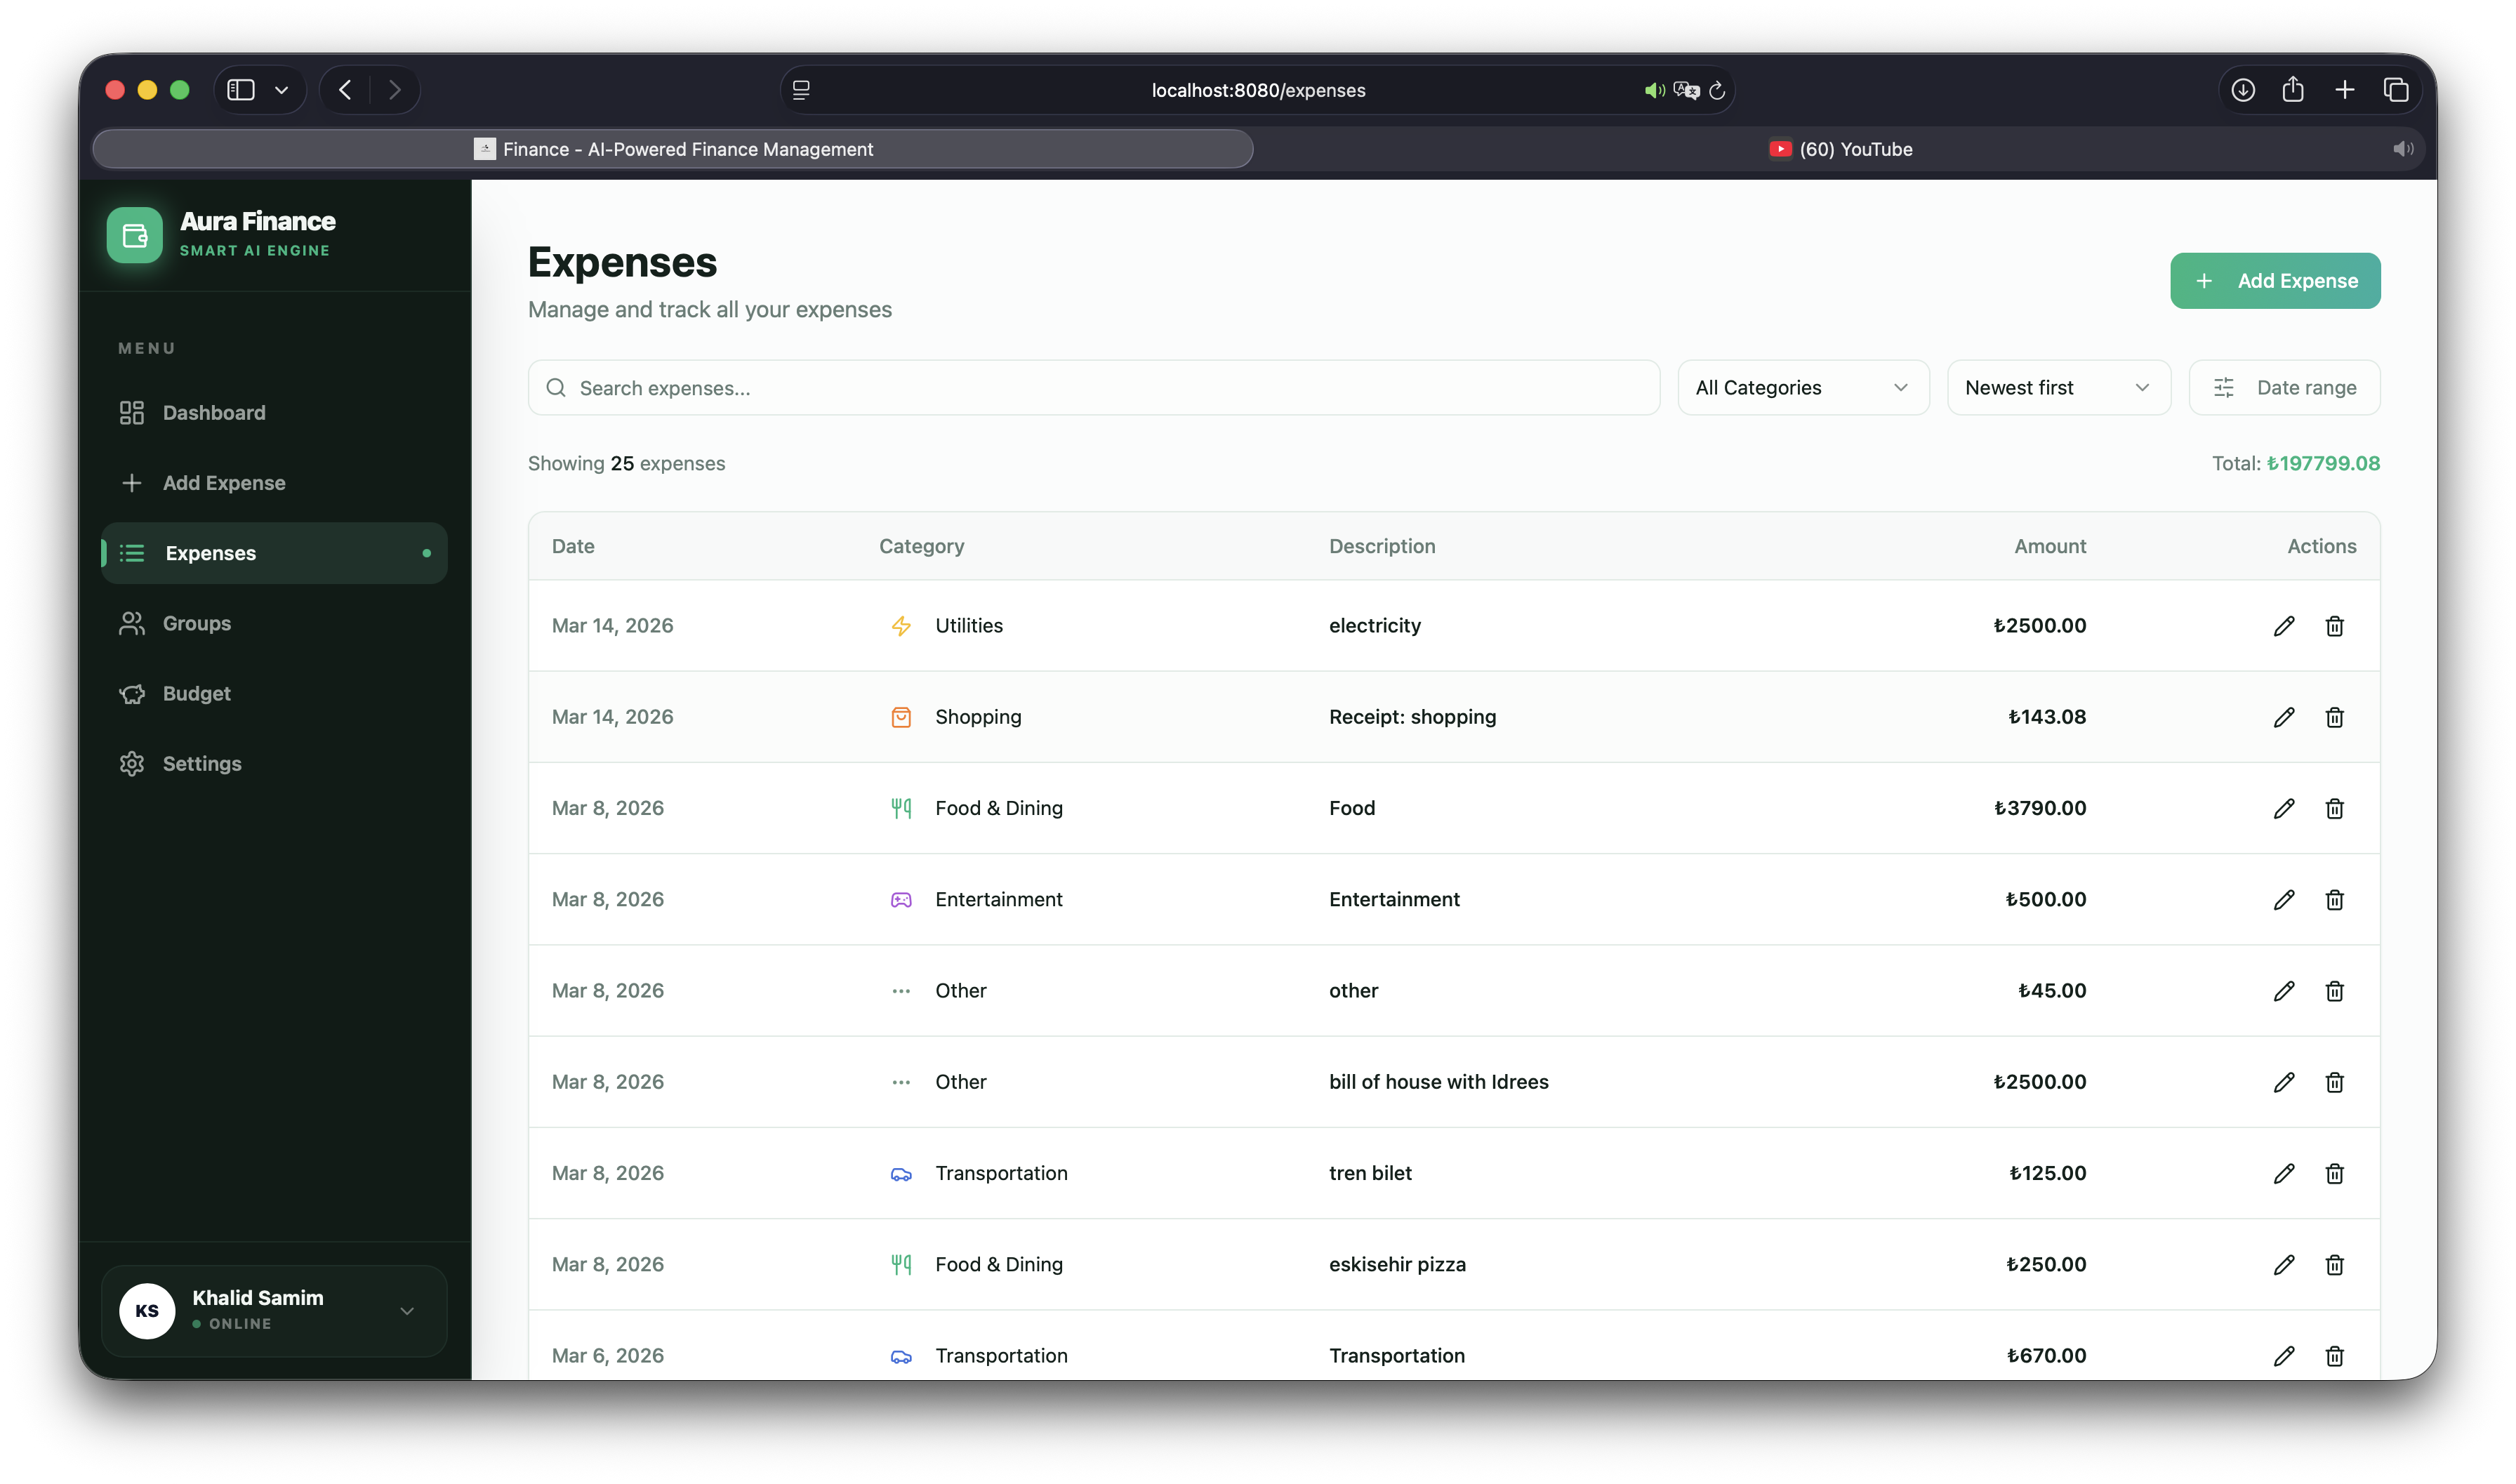
\includegraphics[width=0.8\textwidth]{./fig/aura_sc6}
 \caption{Grup Yönetimi: Yeni Grup Oluşturma Arayüzü.}
 \label{fig:sc6}
\end{figure}

\begin{figure}[h!]
 \centering
 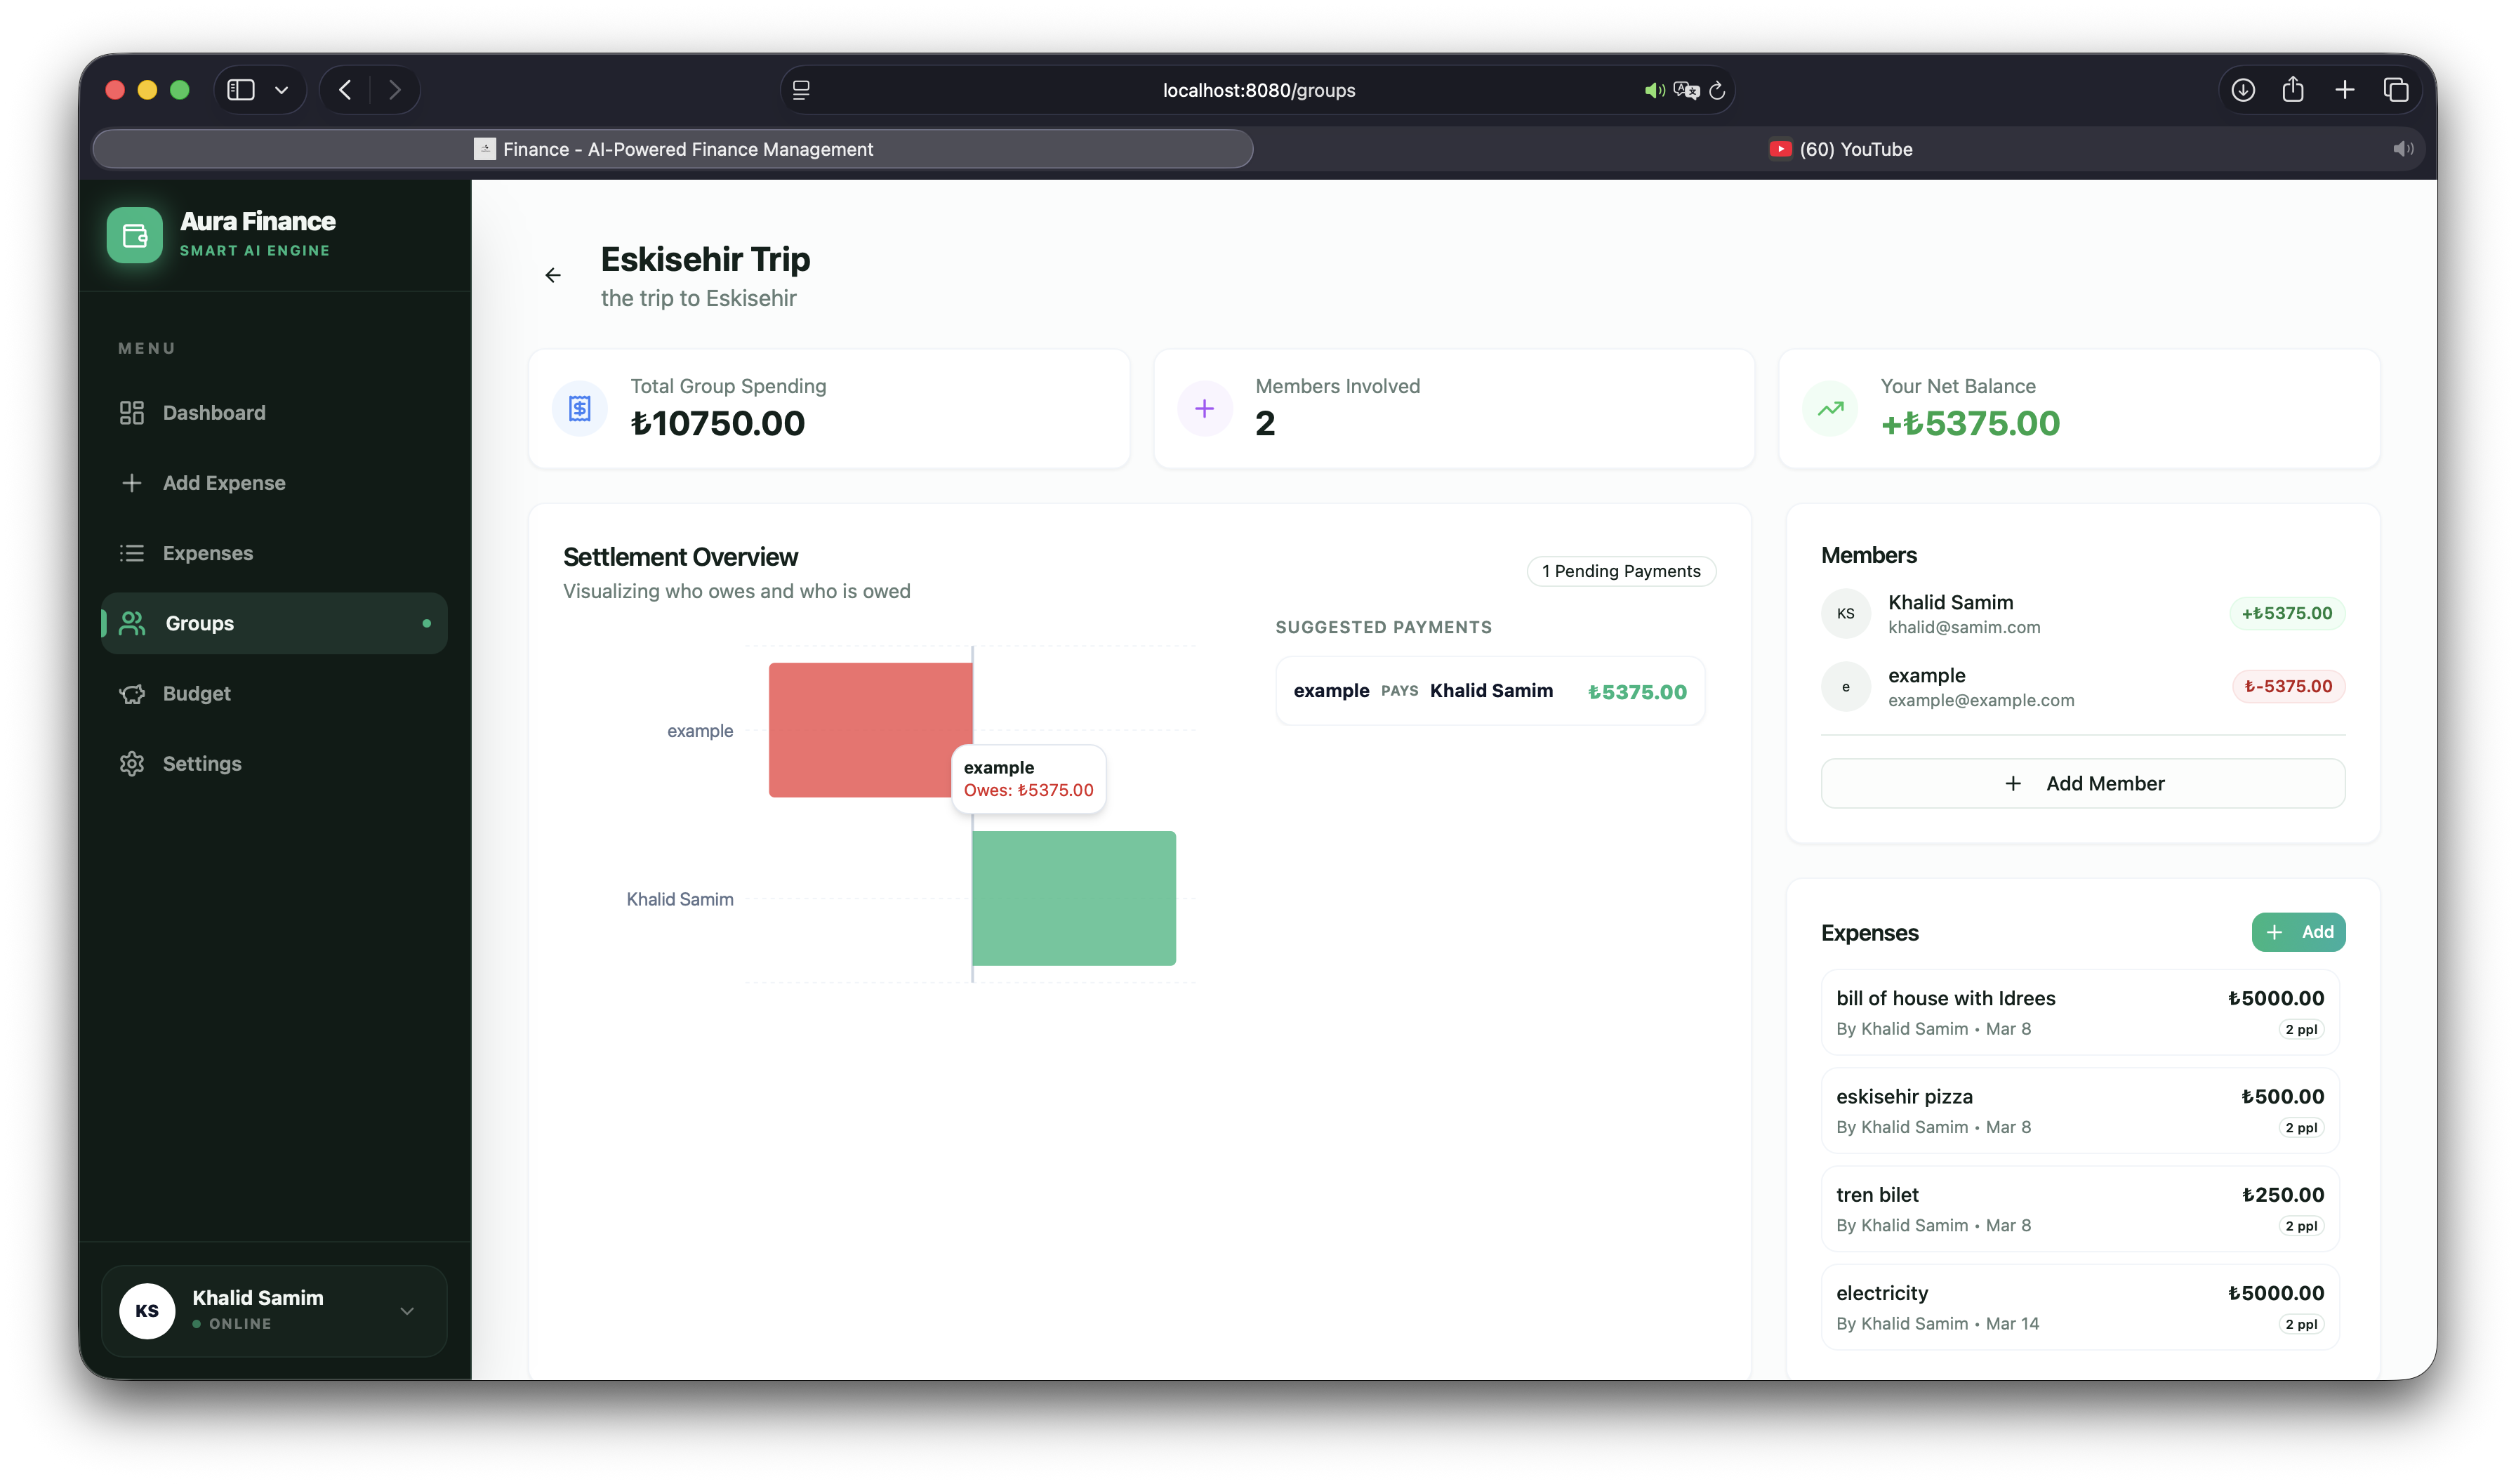
\includegraphics[label=sc7, width=0.8\textwidth]{./fig/aura_sc7}
 \caption{Grup Harcamaları ve Adil Paylaşım Takibi.}
 \label{fig:sc7}
\end{figure}

\begin{figure}[h!]
 \centering
 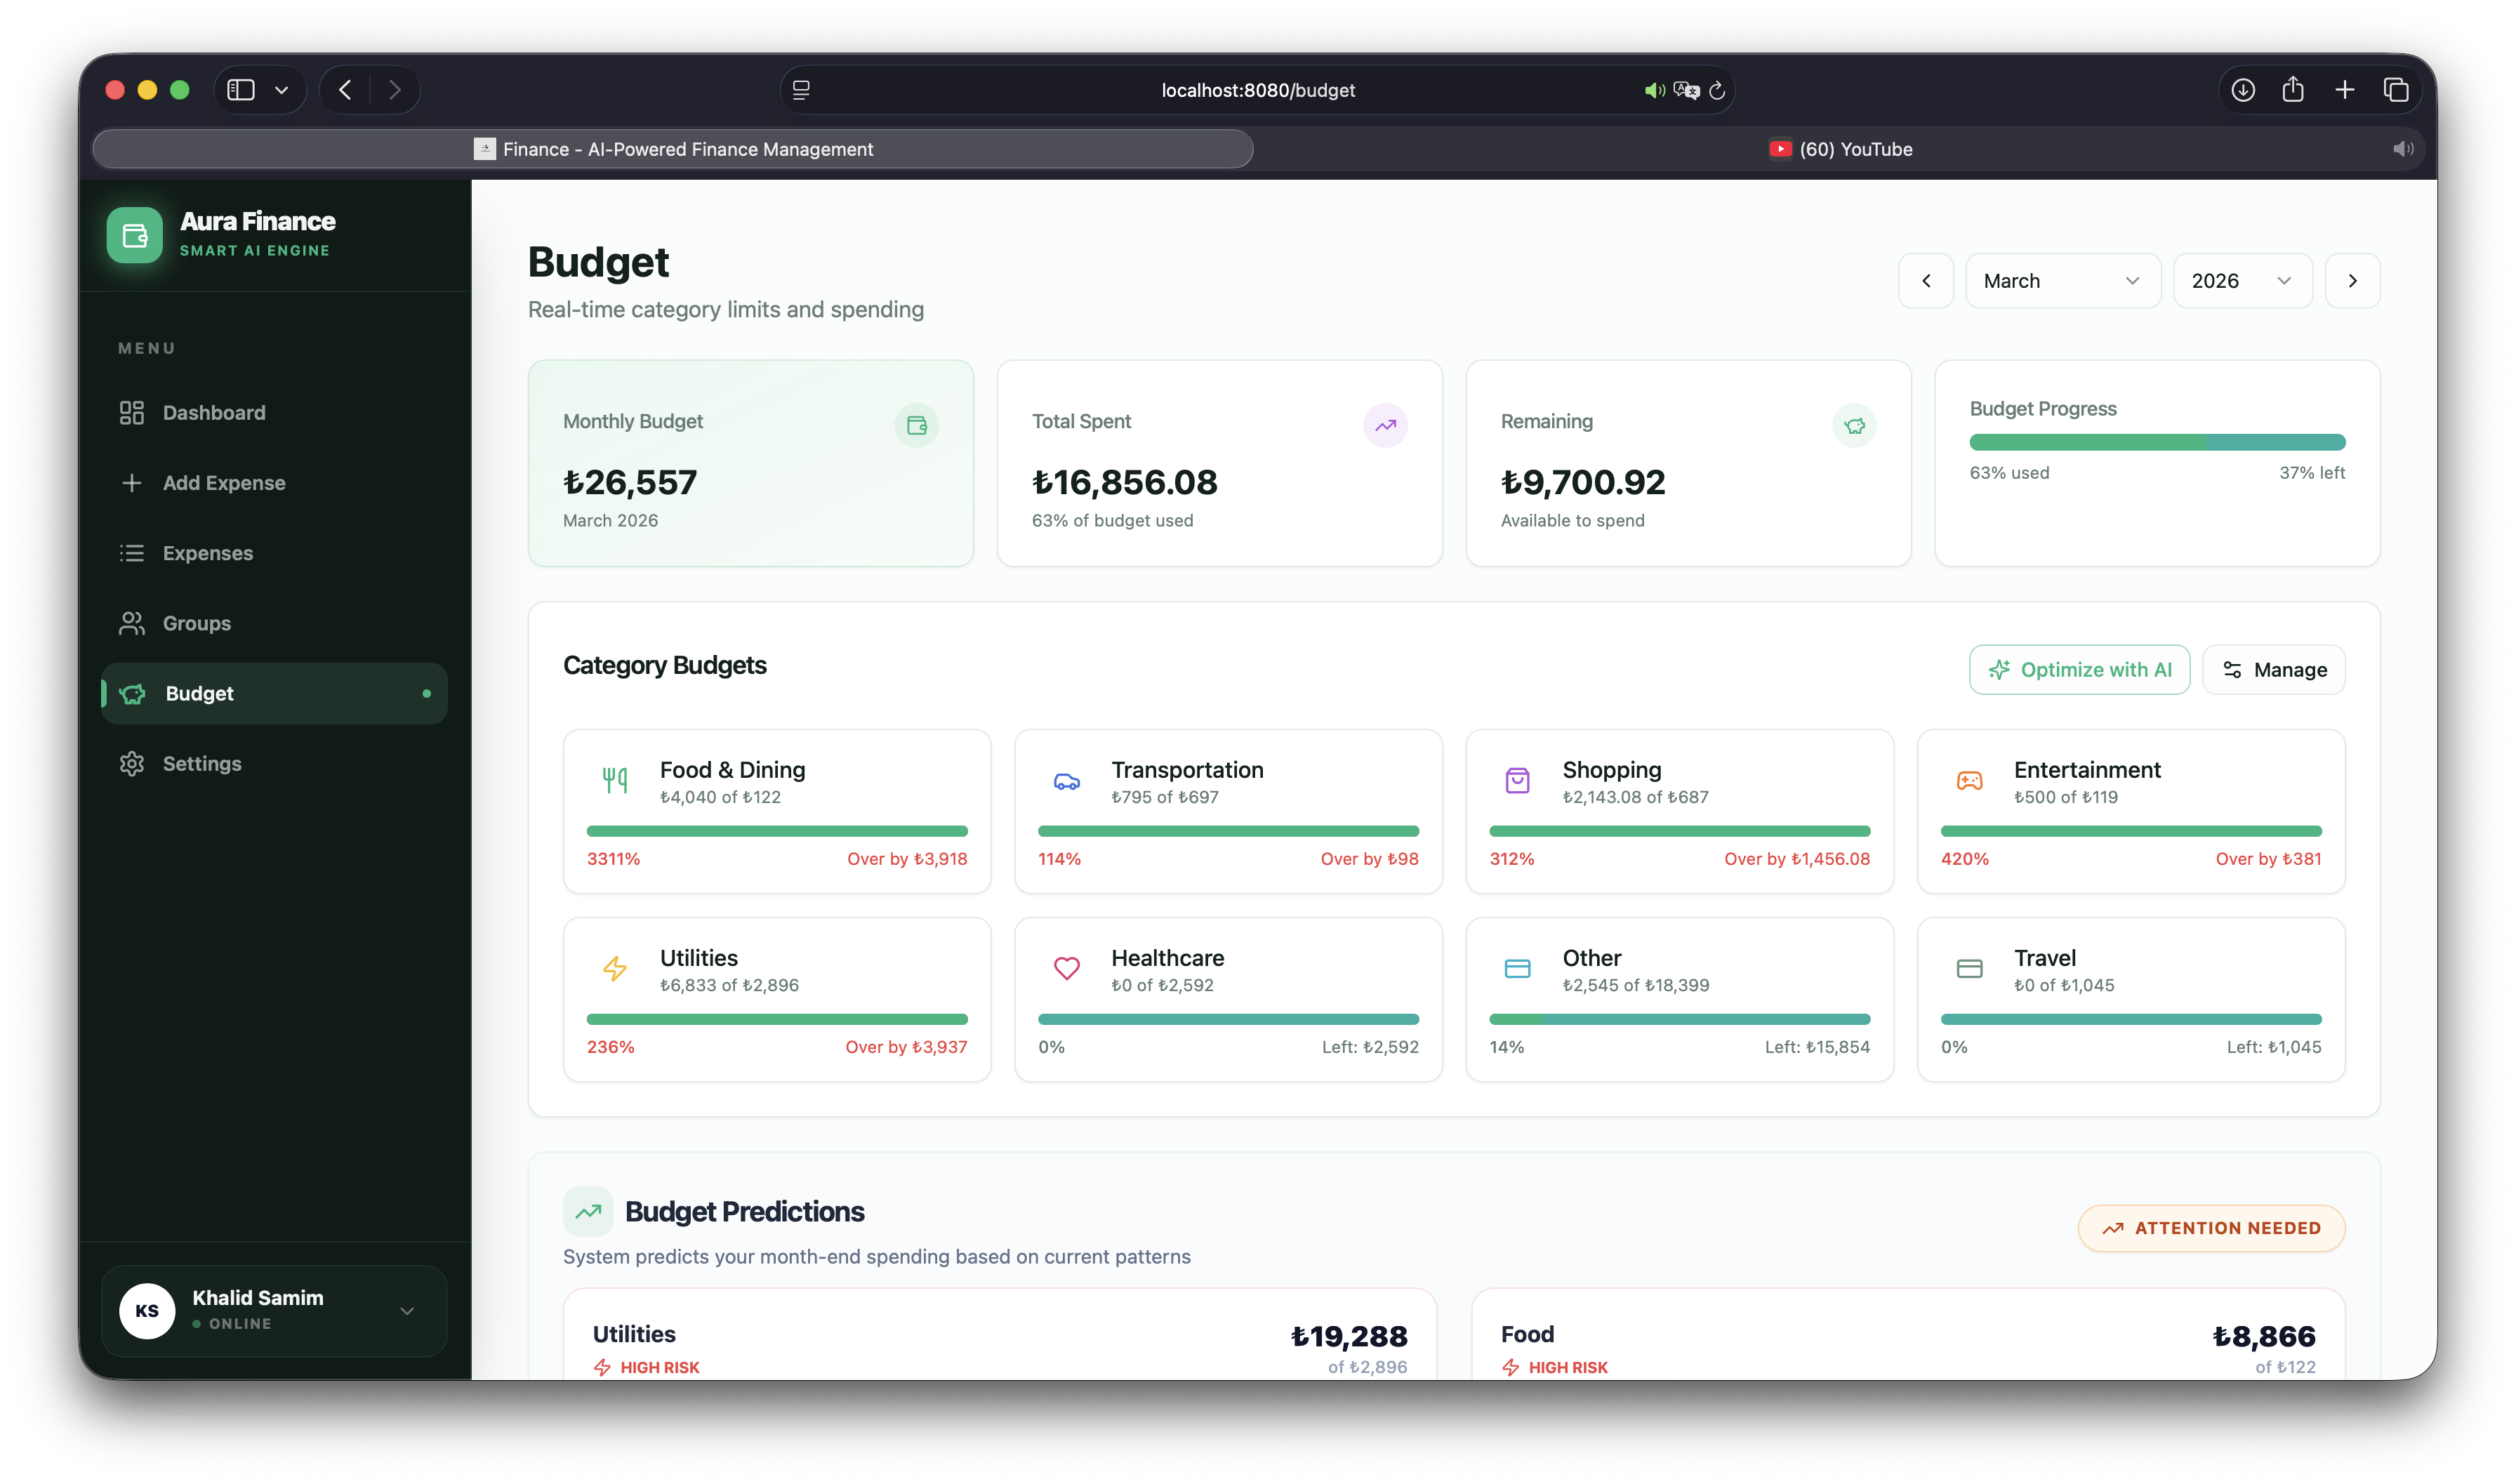
\includegraphics[width=0.8\textwidth]{./fig/aura_sc8}
 \caption{Ayarlar ve Kullanıcı Profili Yönetimi.}
 \label{fig:sc8}
\end{figure}
